\documentclass[12pt, a4paper]{article}
%%%%%%%%%%%%%%%%%%%%%%%%%%%%%%%%%%%%%%%%%%%%%%%%%%
\title{\textbf{The Current State of Spatial Paritioning Trees: A Literature Review}}
\author{Patrick C. Shriwise}
\date{\today}
%\institute{Department of Engineering Physics, University of Wisconsin-Madison, 1500 Engineering Dr, Madison, WI 53706, shriwise\@wisc.edu}

%%%%% packages and defs
\usepackage{setspace}
\onehalfspacing
\usepackage{graphicx}
\usepackage{float}
\usepackage{amsmath}
\usepackage{booktabs}
\usepackage{caption}
\usepackage{epsfig}
\graphicspath{{./images/}{../images/}{./}}
\usepackage[font={small,it}]{caption}
\usepackage{color}
\usepackage{hyperref}
\hypersetup{
    colorlinks=true, %set true if you want colored links
    linktoc=all,     %set to all if you want both sections and subsections linked
    linkcolor=black,  %choose some color if you want links to stand out
}

\begin{document}

\begin{center}
  \textbf{A Monte Carlo Oriented Ray Tracing Kernel} \\
  \bigskip
  by \\
  \bigskip
  Patrick C. Shriwise \\
  \bigskip 
  at the \\
  \bigskip
  UNIVERSITY OF WISCONSIN - MADISON \\
  \bigskip
  2016
\end{center}

\newpage
\tableofcontents 

\section{Abstract}%%Status:Done%%

The value of CAD-Based Monte Carlo relies heavily on the ability to return geometric queries quickly and robustly via ray tracing. The Direct Accelerated Monte Carlo (DAGMC) toolkit currently provides a robust ray tracing algorithm\cite{smith_thesis_2011} given certain mesh requirements are met, but shortcomings of the underlying ray tracing kernel causes it to lag behind run times of a given Monte Carlo code using its native geometric analysis. Up to this point, we have relied on research in ray tracing mainly for the application of rendering or collision detection. Neither of these applications align exactly with the application of Monte Carlo ray tracing. Algorithms for collision detection involves moving geometry which isn’t yet a concern in the area of radiation transport. Algorithms for acceleration structures in rendering typically prioritize the time needed for the building of these structures causing them to be less than optimal, but results in an overall decreased time-to-render due to the balance of the build time with the number of ray queries needed to generate the desired graphics. In radiation transport, the number of ray queries needed to generate the desired result is much larger than the number needed for rendering. As more time is spent ray tracing, the build times of the underlying acceleration structures becomes less significant, thus the balance between time spent building these structures and the time using them for ray tracing must be reconsidered in this context. Its is hypothesized that in the case of the large, complex problems for which DAGMC is intended, that extra time spent optimizing the ray tracing acceleration structures via adaptation to certain mesh features and/or mesh refinement/alteration if necessary. This shift in priorities regarding the building process is important, but there are other improvements to be made as well. An area where the application of rendering and radiation transport align very well is in the query process after building of acceleration structures is complete. There are many advancements in ray tracing techniques which can be applied in order to provide further improvements to DAGMC’s performance. It is hoped that the combined effect of these improvements will bring DAGMC’s performance close to that of the native Monte Carlo codes it supports, thus alleviating the concern for additional computational time while maintaining the benefit of reduced human effort in radiation transport on complex geometric models.

\section{Introduction}%%Status:Done%%

%% The purpose of this document is to outline the current state of the art in spatial partioning hierarchies for the purpose of improving performance in DagMC. It will take into account as much of the existing literature as possible. An analysis of the literature will also be conatined, identifying areas for improvement within the context of ray tracing for the specific application of Monte Carlo ray tracing.

Monte Carlo methods are a class of algorithms employed to solve complicated physical systems or mathematically complex problems which are difficult or impossible to solve analytically. As such, these methods have been employed for the purpose of solving 3D neutron transport problems for real-world systems. In the Monte Carlo process, the path and energy of particles are tracked from their birth until their termination through a series of randomly-determined collision events which are collectively defined as the particle's history. If a particle is scattered during one of these events, its direction and energy changes and it moves on to the next collision or event. If the particle is absorbed or escapes the system, the particle's history is terminated. Throughout this process, the material or volume in which the particle exists will will determine physical quantities which influence the randomly-selected events the particle encounters. As such, it is necessary to know when the particle is moving from one volume to the next through out its lifetime. In the organization of most Monte Carlo codes, an event arises in the particle's history and the distance to this event along the particle's direction from its current position is determined. It is then important to know whether the location of the particle's next event lies inside or outside of the volume in which the particle currently exists. If the event location lies inside the volume, then the particle can step forward to that location and the event will be recorded as part of that particle's history. If the event location lies outside of the volume, the event cannot be considered valid as it could be taking place inside of a material with different physical properties with respect to the particle. In this situation, the particle is then moved forward to surface of the current volume and is logically place inside of the volume on the other side of that surface. At this point the particle's history continues and its next event will be selected. In order to determine if the event location lies inside the current volume, the closest distance to the boundary of the volume along the particle's current trajectory must be found. The specific queries of interest being the closest surface intersection to a particle's location and the closest surface intersection to a particle's location along its current trajectory. The tracking of particles through the virtual space of a model occupies is a problem commonly encountered in the area of computational modeling and there are many approaches to this problem, each having its own advantages and disadvantages.

Most Monte Carlo geometries come in the form of Constructive Solid Geometry (CSG). CSG allows one to form a complex volume from a set of Boolean operations on CSG primitive objects such as cylinders, spheres, parallelepipeds, etc. CSG allows for an exact representation of these objects via analytical forms for each of these objects. This in turn allows for the direct calculation of the nearest surface intersection by performing intersection checks for each of the CSG objects of which the volume is comprised and using the smallest of these values. Given that these checks can be done using some analytical form, the necessary geometric queries required for Monte Carlo can be returned quickly to the physics code throughout the particle's history in $O(N)$, where N is the number of primitive objects used to define the volume. Historically, there are limitations associated with the use of CSG as a geometry representation also. First, there is a practical limit to the complexity of volumes that can be formed using CSG objects. Volume formations require human knowledge and verification of the primitive object combinations required to form each volume in the CSG model. Given that in most current implementations these models are formed via a text-based implementation, highly complex volumes can be extremely difficult to create and modify. As a result, a large amount of human time is spent generating and verifying modules of complex real-world systems. In reality, there are volumes which are impractical to represent due to the difficulty of their representation via CSG. These objects are typically modified in Monte Carlo models as an approximation of the real volume, each approximation or feature removal requiring its own justification for its affect on the outcome of the desired solution. The consequence of this in the broader scope of engineering analysis is that different models are being used for structural, thermal hydraulic, magnetic, etc. analysis. Many of these other types of analysis already take advantage of CAD systems for their geometry representation, allowing better representation of the as-built systems and faster design iteration for geometry-related alterations. Based on the established methods of these other types of analysis for CAD-based models, this provides significant motivation for radiation transport on CAD models as well.

The use of CAD models allows for radiation transport on arbitrarily complex models - allowing one to almost exactly represent real-world systems. Though as the geometric representation becomes more sophisticated, particle tracking during transport becomes more complex. Analytical forms of CAD surfaces and volumes are sometimes impractical or impossible to compute over entirety of the object's domain. To circumvent this problem, surfaces are triangulated to provide a generalized representation for each surface as a triangle mesh. All geometric queries from the Monte Carlo code can then be handled the same way despite the volume's form or complexity. Robustness can also be a challenge when using CAD based models, often times caused by poorly defined mesh topology at surface interfaces. It has been shown, however, that transport using CAD models can be equally as reliable as that of CSG based systems can be achieved \cite{smith_thesis_2011}, and it is worth mentioning that these triangle mesh's are generated such that all points on the mesh are within a specified tolerance of the analytical representation of the surface, meaning that all significant features of the model are intact during transport. The performance of such CAD based systems is lacking in comparison to that of most CSG based codes, typically several times slower in production models. In part, this is caused by the triangulation of surfaces. The problem of finding the closest or next primitive object of intersection is now more difficult due to the sheer number of triangle primitives needed to represent complex models. However, the problem has now been reduced to a well-researched problem known as ray tracing. Ray tracing is most commonly used to generate 2D images by simulating light ray interactions with virtual 3D objects in a process known as rendering. These light rays (photons) are typically cast from the perspective of the image to be generated, and pixel colors are determined by the reflections, refractions, etc. of the photons on their course to the light source. This process is a naturally analagous to Monte Carlo analysis despite the vastly differing physics behind the final solution. In realistic renderings, it is sometimes possible that light rays may scatter before reaching the next virtual object on their path. In order to determine if this will occur before reaching the next object, the distance to interaction (scattering or otherwise) must be compared to the distance to the next object just as in the Monte Carlo process for radiation transport. For highly complex models, a linear search of the primitives is out of the question in terms of computational expense when models may require millions of triangle primitives. As a result, extensive research has been done in the area of acceleration data structures for ray tracing which section the problem space in order to establish a binary tree-like search over the geometric primitives of the model. Using acceleration datastructures oriented toward these spatial searches, geometric queries can be satisfied in $~O(log(T))$ time, where T is the number of triangles needed to define the volume.

The acceleration datastructures currently used in CAD-based systems were adapted from work on object interference detection in 1996\cite{gottschalk1996obbtree}. This particular datastructure is a binary hierarchy of oriented box bounding volumes used to rapidly reduce the number of primitives in the geometry query to a small set which are then tested for geometry query of interest. This datastructure was chosen for the relatively shallow hierarchy it produces so that it may work well within a mesh database framework which is not necessarily oriented toward binary search performance. Recent work in the area of ray tracing in conjunction with the re-emergence of common chipset architectures oriented toward single instruction multiple data (SIMD) implementations has increased the performance of CPU based ray tracing kernels significantly \cite{wald_simd}, allowing a proof of concept for CAD based radiation transport which is on the order of CSG based implementations.

This document will discuss the background and theory of several different areas surrounding particle tracking in CAD-based Monte Carlo, the current state of ray tracing acceleration datastructures, and other optimization techniques of interest for particle tracking in Chapter \ref{background}. Chapter \ref{perf_benchmark} will examine the descrepancy in performance between the current state of CSG anc CAD geometries in more detail. Next, a particularly problematic feature seen in CAD-based meshes will be characterized and addressed in Chapter \ref{hv_study}. Then a proof of concept for CAD based Monte Carlo competitive with that of native codes will be presented in Chapter \ref{emdag}. Finally, a new approach to ray tracing for CAD based systems in Monte Carlo will be proposed in Chapter \ref{research_proposal}.

%% In fact, the specific problem of finding the next closest intersection within a virtual model given a point and a direction is commonly encountered in the area of rendering for 3D models.

%%  As a particle is born, the material in which it exists must be determined as it will dictate the underlying physics of its travel through 

%% The (DAGMC) toolkit \cite{dagmc_2009} robustly tracks particles through geometries represented by a surface mesh provided by the graphics faceting of the CAD engine in which the geometry is generated. Thanks to the make\_watertight algorithm\cite{make_watertight_smith_2010} DAGMC can robustly track particles through highly complex geometries by providing the necessary geometric information to underlying Monte Carlo physics codes via a ray tracing kernel in the Mesh Oriented dAtaBase (MOAB)\cite{moab}. This geometric information typically comes in the form of the distance to next surface and particle in cell queries. This process has allowed for successful transport runs of complex models of the International Thermonuclear Experimental Reactor (ITER) for runs upward of 1E8 histories with zero lost particles.\cite{smith_thesis_2011}

%% Naturally following the ability to do these robust calculations on already complex models, increasingly detailed models are becoming of interest. Unfortunately it has been shown that as detail increases, the performace of DAGMC lags more and more in comparison to the native versions of the various Monte Carlo codes it supports (see Table \ref{DAG-MCNP_performance}). It is known that this performance issue is due to the time it takes to return geometric information to Monte Carlo packages from the ray tracing kernel it relies upon. Historically this has been true of applications which rely on ray tracing processes.\cite{Intro2RT} In agreement with this trend, this work shows that ~85\% of the run time of DAGMC baed transport is spent in the ray tracing kernel. The remainder of this work details an investigation into the shortcomings of DAGMC's ray tracing process as well as various options for improvement. An important part of this investigation is the analysis of ray tracing from the application-specific perspective of its use in Monte Carlo radiation transport.

%% \begin{table}[H]
%%   \centering
%%   \caption{Table comparing the performance of DAG-MCNP to native MCNP for the same modules after translation to a CAD-based surface mesh.}
%%     \label{DAG-MCNP_performance}  
%%   \begin{tabular}{l c c c}
%%     \toprule \\
%%     Model & Native ctme (min) & DAGMC ctme (min) \\
%%     \hline \\
%%     FNG &  5871.92 & 22769.33 \\
%%     ATR &  901.68 & 8627.80 \\
%%     UWNR &  8767.29 & 69429.60 \\
%%     \hline \\
%%   \end{tabular}
%% \end{table}


%% Each of the ray tracing kernels studied later in this work were initially intended for other applications and adapted for use in Monte Carlo. MOAB's Oriented Bounding Box (OBB) hierarcy was initally designed for use as part of an interference detection algorithm\cite{gottschalk1996obbtree} while Embree (discussed later) is a ray tracing kernel optimized for the purpose of interactively rendering static or dynamic models. Ray tracing in Monte Carlo differs from each of these applications though it is more closely aligned with the process of rendering than interference detection. Even so, Monte Carlo ray tracing differs from rendering in a fundamental way and deserves to be approached uniquely rather than as an adaptation or extension of another purpose. This is true for a few different reasons.

%% In Monte Carlo, a significantly higher number of ray queries are made than in rendering. In order to obtain a statistically valid anser to the problem at hand, the number of primary is generally an order of magnitude higher than that of a rendering problem. The average number of secondary ray queries is even more so. In radiation transport, interactions may occur at any point in space (depending on the virtual material which occupys that space) rather than nearly always at the interface of object. This increased spatial interaction frequency leads to a much larger number of secondary ray queries ($O(100)$)than one might or could see in a rendering process. In either case, the time to solution (render) can be roughly described by the time needed to construct the necesary acceleration structures and satisfy the ray queries.

%% \begin{figure}[H]
%%   \centering
%%   \caption{A rough estimation of the number of ray queries in a typical rendering vs. in the FNG model runs. The number of pixels per ray was determined by common practice in rendering.}
%%   \label{render_ray_estimate}
%%   \[ (8\, rays\, per\, pixel)\, x (1024 x 1080\, pixels) = 16.6M \, rays \]
%% \end{figure}


%% Time it takes to perform the ray tracing queries is partially dependent upon the quality of the acceleration structure being built. The better the quality of these structures is the faster the ray queries will be satisfied and the solution reached. The quality of the accceleration datastructure is also dependent on the amount of time spent in building the datastructures. Presumably the more time spends building the datastructure, the better its quality. Typically, rendering tools focus on building a generalized data structure with respect to the mesh its operating on without consideration of the more subtle features of the mesh and how the datastructure's quality might be improved. This is commonly because the time spent in improving the quality of the datastructure is overly costly compared to the total amount of time saved when performing the ray queries. In the scenario of Monte Carlo, it has been established that many times the number of rays are being fired in order to obtain the solution several times over. In this case the saved time in performing necessary ray queries may then become significant, and that the extra time spend in building the acceleration datastructure to increase its quality becomes favorable. The trade offs of these costs/savings are difficult to quantify in that (as is the case for most ray tracing performance evaluations) they vary greatly model to model. However, the severe degredation in ray fire times due to mesh features produced by the surface mesh generation algorithm on which DAGMC relies leads one to believe that adapting to such mesh features and any other such features discovered in the future is worthwhile.

%% \begin{figure}[H]
%%   \centering
%%   \caption{General equation for the time to solution of a ray tracing based process.}
%%   \label{tts_eq}
%%   \begin{align*}
%%     tts =\, & C + T_{B} + \sum_{}^{N_{r}} T_{T} \\
%%     tts =\, & C + T_{B} + \sum_{}^{N_{r}} T_{T}(q,\ldots) \\
%%     q(T_{B}) & \rightarrow T_{T}(T_{B}) \rightarrow T_{T} \propto \frac{1}{{T_{B}}^{x}} \rightarrow x \geq 0 \\
%%     tts =\, & C + T_{B} + \sum_{}^{N_{r}} T_{T}(T_{B},\ldots) \\
%%     tts - & time\, to\, solution \\
%%     C - & cost\, of\, other\, operations \\
%%     T_{B} - & acceleration\, datastructure\, build\, time \\
%%     T_{T} - & average\, traversal\, time \\
%%     N_{r} - & rays\, required\, for\, solution \\
%%     q - & acceleration\, datastructure\, quality \\
%%   \end{align*}
%% \end{figure}

%% Additionally, the way in which rays traverse a model limits the number of possible triangles for a given ray query to the triangles used to form the current volume (cell) in which the particle resides. As a result, trees are created on a per-volume basis whereas in rendering rays are allowed to hit any object in the virtual space. This difference in perspective a manifestation of the underlying physics between the two applications. Most interactions of influence occur inside virtual objects of non-negligible density rather than in the relatively empty space between them. In rendering, most of the interesting interactions affecting the blurring of objects, shadowing, etc. occur in this void or air-filled space between objects.

%% Many ray tracing datastructures, heuristics, and other techniques are explored as part of a review of ray tracing's current state. This is followed by an analysis of DAMC's performance limitations as well as the investigation of known problem-specific difficulties encountered by ray tracing kernels as a result of the process used to generated surface meshes in the DAGMC workflow. Finally a plan is laid out to create a Monte Carlo oriented ray tracing kernel which couples the existing functionality of current tools such as MOAB with some of the more powerful ray tracing techniques currently available and seeks to take advantage of more subtle optimizations specific to its purpose.


\section{Background}%%Status: In Progress%%
\label{background}


\subsection{Acceleration Datastructures for Ray Tracing}

Acceleration datastructures for ray tracing are designed to rapidly narrow the search for a location in virtual space given a starting position and orientation. This is accomplished by sectioning the space using a partitioning construct in either the spatial or entity dimension. The paritions are determined by a division heuristic which establishes the partitions given a set of primitives. After partitioning, the primitives are then associated with the partition in which they are contained. This process is recursively repeated until leaf conditions are met. This can be based on the remaining number of primitives, the current size of the partition, or by other means. The end result is a hierarchy which can be used to traverse the problem space efficiently for ray intersections or closest intersection queries.

\subsubsection{KD-Trees}%%Status:Done%%

The KD-Tree or multidimensional binary search tree was originally developed as a method for querying records in databases and has since found use in other applications including speech recognition, global information systems, and ray tracing. \cite{Bentley1975} KD-Trees operate by recursively dividing the dimensions of the problem set in a spatial manner. At each level of the tree a different dimension is spatially split. Typically the tree will cycle through the dimensions of the virtual space for different levels in the tree. The resulting subsets of this split are labeled as children of the parent set and the process continues until leaf conditions are met. Entities are listed as contained by a partition only if they are contained by all parents of the partition as well, meaning that all entities lie within some subset in each dimension of the problem.

This process is easily applied to the virtual 3D space of CAD models for ray intersection queries. The problem space is divided evenly in the x dimension. The two child partitions are then divided along the y axis and the resulting children of this division are subdivided along the z axis. Divisions are typically done s.t. the space of the current candidate is separated in half, however it is possible that by doing this primitive entities are divided by the hyperplane as well. There two ways that this is typically handled. The first is to simply reference any primitives in both of the subdivisions. This has the effect of creating a small overlap between the partitions, but requires no changes to the original model. The other solution is to divide the primitive entities in two using the division plane. While in terms of data structure traversal, this solution requires alterations to the model which may be undesirable under certain conditions and violates the description of the KD-Tree as a query acceleration structure by making modifications to the existing data.

KD-Trees are frequently citied as being able to provide the best ray tracing performance to date.\cite{ernst_2007} In particular, KD-Trees are noted as being better equipped to handle models with highly varying triangle sizes/densities. Bounding volume hierarcies are currently favored, however, for their lower memory footprints and well-developed parallel building schemes. These features are of great import for systems with limited memory, such as GPUs, and applications with intent for realtime viewing or interaction. These requirements do not necessarily apply to the realm of Monte Carlo particle tracking done on CPUs with more memory available relative to GPUs and less concern for the time spent building acceleration datastructures, however. 

%% 2-D Example from Bentley1975 here %%
\begin{figure}[H]
  \caption{Two dimensional KD-Tree example adapted from Bently 1975[ \cite{Bently1975}. Left: Graph representation of the KD-Tree. HISON's are right children. LOSON's are left childre. Boxes are null. Right: Two dimensional space partitioned in the graph. Boxes represent the range of their respective subtree.}
  \label{2dkd}
  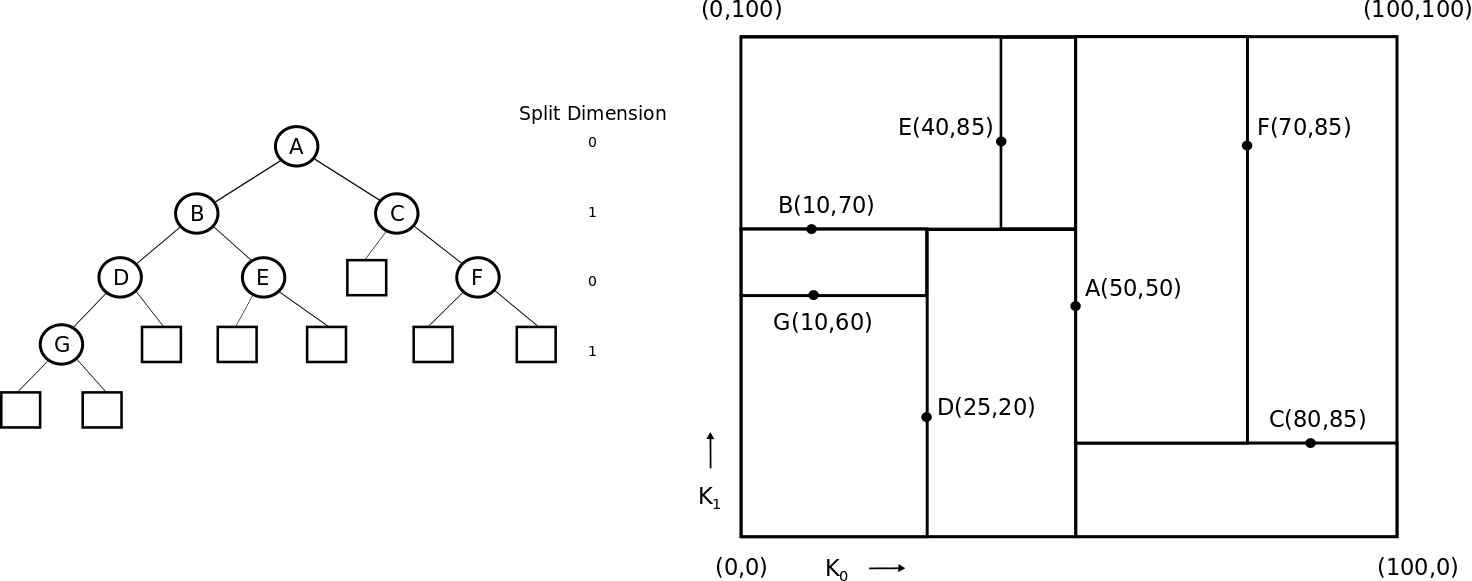
\includegraphics[scale=0.25]{2d_kd_eg.png}
\end{figure}

KD-Trees are able to out-perform many other acceleration datastructures due to traversal schemes developed based on the inherent quality of KD-Trees having non-overlapping sibling nodes. As a KD-Tree is being constructed, an ever-shrinking bounding box is being defined as one moves deeper into the tree. At the leaves of a KD-Tree a well-resolved bounding box can be conceptualized using the coordinates of the last 6 splitting plane coordinates, two in each dimension. Due to the nonoverlapping quality of the KD-Tree nodes, the faces of this bounding box can be linked to spatially-adjacent nodes in the tree. These links are referred to as neighbor links \cite{KDReview} and can be used to significantly reduce traversal costs. During traversal, if a leaf is visited its neighbor links can be used to direct the query to either the next adjacent leaf or a nearby interior node in the tree thus avoiding a depth-first style traversal in which the next step upon visiting a leaf node is to return to the root node of the tree and continue. These neighbor links take advantage of the idea that if a leaf node is visited, but the desired intersection is not found, then it is likely that the desired intersection is close to the current leaf location. In this way, one can avoid large amounts of shallow-level tree traversal.  

\subsubsection{Bounding Volume Hierarchies}%%Status: Done%%


Bounding volume hierarchies (BVHs) are currently the favored datastructure in the field of rendering. 

The initial concept of using the bounding volume construct as a pre-check for ray-intersection with objects was introduced by Weghorst in 1984 \cite{Weghorst:1984:ICM}. Weghorst explored the possibility of using spheres and rectangular parallell pipeds (boxes) to contain geometric objects. This work also went so far as to create a hierarchy of those object-based bounding volumes, noting the importance of hierarchicaly joining bounding volumes near to each other in space so as not to have parent volumes containing large amounts of empty space between the volumes to be joined.

\begin{figure}[H]
  \caption{Two dimensional BVH example adapted from Gottschalk 1996 \cite{gottschalk1996obbtree}}
  \label{2dbvh}
  \centering
  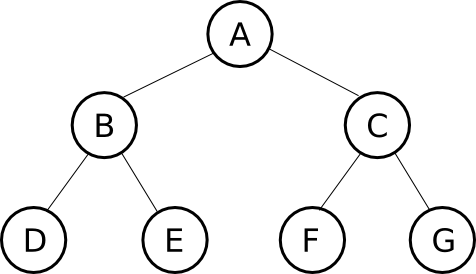
\includegraphics[scale=0.3]{binary_graph.png}
  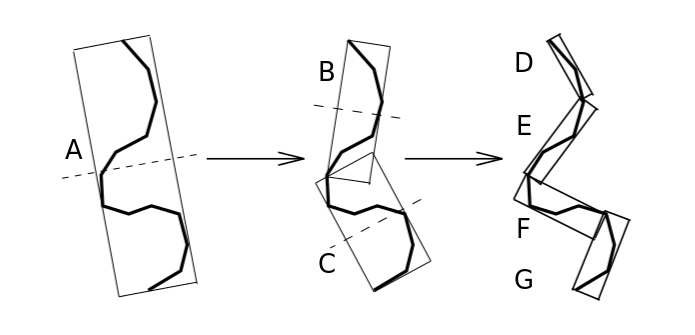
\includegraphics[scale=0.3, trim = 0 50 0 0 ]{bvh_2d_ex.png}
\end{figure}

As CAD systems improved, it was found that complex geometric objects become difficult to render as the analytic calculation of ray intersections became more costly. As a result, representations of geometric objects were then triangulated for rendering purposes. Ray interactions with these more simple triangle primitives are much less costly to compute in comparison to the previous analytic representation. Given that the geometric object can be discretized accurately, this also allows for the rendering of arbitrarily complex geometric objects without the need for continuous development of efficient analytic intersection techniques for all classes of complex parametric surfaces. 

Hierarchies of bounding volumes could then be created on subsets of the primitives, making even more effective accelerations of ray tracing.

In Weghorst's exploration of sphere and box bounding volumes it was found that while spherical bounding volumes are less compuationally expensive to check for ray intersections than bounding boxes, the latter generally provide a tighter fit to the objects they contain. This tighter fitting is important as it decreases the chance of wasted intersection checks for rays which intersect the bounding volume but not the primitives it contains. This becomes particulartly important as BVHs become deeper when subdividing on many primitive entities and more intersection checks are performed. Even applied to analytical objects, this affect was reflected in the results of Weghorts's work strongly enough to show that bounding boxes were significantly more effective in accelerating the ray intersection process than bounding spheres. Two forms of BVHs have been applied in ray tracing problems: axis-aligned bounding boxes (AABBs) and oriented bounding boxes (OBBs).

AABBs are boxes whose orientation is restricted such that their faces are parallel to the global planes of the problem space. In practice, tightly fitting axis aligned boxes are straightforward to construct given a set of points to contain, and overlaps between the children of a parent box are minimal. Their simplicity results in a relatively low memory footprint and simple, robust ray-intersetion tests. Unlike axis aligned bounding boxes, the faces of OBBs are allowed take any orientation relative to the global axes in order to enclose their set of primitives as tightly as possible. There are several existing methods for determining the orientation of a box for best fit to a set of primitives.\cite{gottschalk1996obbtree} As a result, oriented bounding boxes are better for avoiding erroneous ray-box intersections that might otherwise occur for an axis aligned box, and they more quickly conform to the full set of enclosed primitives as the boxes are subdivided. This conformity leads to more shallow hierarchies making the worst case number of intersection tests lower than for an axis aligned box hierachy on average. While a shallow hierarchy might indicate a smaller memory footprint, OBBs require one to store some extra information about their orientation relative to the global axes making this assumption difficult to consistently prove. One distinct disadvantage of oriented boxes encounterd upon hierarchy traversal is that the intersection check requires an extra step in transformation of the ray to the oriented axes of the box in question. The information needed for this basis transformation of the ray must be constructed and applied to the ray before the box intersection can continue as it would for an axis aligned box. So while the oriented box hierarchy may have fewer intersection checks to do for a given ray query than an axis aligned box, the intersection checks are inherently more expensive than in the case of AABBs. In practice, AABBs are commonly used in BVH's for their simplicity of implementation and well-researched ray intersection algorithms. Other reasons for this preference will be discussed later in this work.

There are a couple different approaches to constructing such datastructures given a set of geometric primitives, but only top-down approaches will be discussed here. The top down approach begins with a single bounding volume encloses all primitives. At this point, child boxes of this root volume are created by selecting a splitting plane for the box which divides the primitves contained by the current bounding volume into two subsets. This process is then repeated until conditions are such that is is disadvantageous to create children of the current node. These conditions are typically referred to as leaf conditions due to the termination of the tree's branch at that node. The selection of candidate splitting planes and the selection of a final plane for splitting based on its estimated worth can greatly affect the performance of the datastructure. A virtually infinite set of planes could be tested to find the optimal plane for dividing the entities between the two child volumes, but even if one were to encounter such a splitting plane, it can be difficult to discern that this is the case. As a result, a limited set of planes is tested for the best split based on a set of assumptions about the problem and some heuristics shown to provide the best performance. The most common method for split plane candidates is median plane splitting in which a bounding volume is split in half for each axes of the current bounding volume. The splitting planes are then evaulated and the best plane is selected based on some estimation of its performance based on some heuristic. The most effective heuristic used in interactive ray tracers today is the surface area heuristic (SAH).

This heuristic provides a way to select the best split of a set of split planes and determine if current node has met the leaf conditions of the hierarchy. The surface area heuristic uses the surface area of child bounding volumes relative to the current bounding volume's surface area as an approximation for the probability that the child will be visited after the parent volume. The explicit form of the surface area heuristic was introduced in 1987 by Goldsmith and Solmon \cite{goldsmith_1987} and later formalized by MacDonald and Booth in 1990 \cite{macdonald_1990}. Its full form is:

\begin{figure}
  \caption{Full form of the surface area heuristic.}
  \label{SAH}
\begin{centering}
  \begin{align*}
    C = & \,C_{t} + \frac{SA(B_{L})}{SA(B)} |P_{L}|C_{i} +  \frac{SA(B_{R})}{SA(B)} |P_{R}|C_{i} \\ C_{t} - & \,cost\, of\, traversal\, to\, child\, nodes \\ C_{i} - & \, cost\, of\, primitive\, intersection\, check\, \\ SA() - & \, gives\, surface\, area\, of\, bounding\, volume \\ B_{L} - & \, bounding\, volume\, of\, left\, child \\ P_{L} - & \, primitives\, contained\, by\, the\, left\, child  \\ B_{R} - & \, bounding\, volume\, of\, right\, child \\ P_{R} - & \, primitives\, contained\, by\, the\, right\, child \\ B - & \, parent\, bounding\, volume
  \end{align*}
\end{centering}
\end{figure}

So the cost of each split done in the tree is assessed as the cost of an extra traversal downward in the tree, as well as the cost of the intersection checks for each primitive contained by the child nodes as if they will become leaf nodes. Both of the children will not always be intersected by a ray however so the cost is then adjusted by some estimation of the probability that a ray which intersects with the current volume will also intersect with a given child volume. In the surface area heuristic this probability is estimated as the surface area of the child bounding volume divided by the surface area of the parent volume and the cost of the primitive intersections are weighted as such. In reality, a better estimation of  child node intersection probability would be given by the relative cross section of the child/parent bounding volumes with respect to the ray direction. Given that ray directions are unknown a priori, the surface area serves well enough for applications with uniform ray distribution. This heuristic is used to produce the highest qualti BVH's achievable by today's standards and now generally regarded as the best method in many production ray tracers today.

One difficulty that bounding volume hierarchies of any type face is that of overlapping sibling bounding volumes. Overlapping sibling volumes can cause additional box intersection checks in a similar manner to loosely fitting bounding volumes. If a ray enters a region of overlapping sibling volumes, this causes the children of both boxes to be checked despite the fact that the ray will eventually only intersect with the desendants of one box or the other. Overlaps are difficult to avoid, however, due to the reality that volumes are required to contain discrete elements for robustness, not just a section of the virtual space. Simply put, if the splitting plane of a bounding volume goes through one of the geometric primities, there will be an overlap in the resulting child volumes. As one can imagine, this is more often the case than not. This inefficiency can be exacerbated by the structure of triangulated objects the BVHs are being formed around. The overlaps found in axis aligned bounding boxes are typically limited to the size of perhaps one or two geometric primitives. Fortunately, there are ways to cope with this problem.

The spatial BVH variant (SHBV) was introduced by Stich et. al. in 2009 \cite{sbvh}. In this building method, a bottom-up construction method is applied with an additional complexity to the node splitting step. As candidate split planes are considered, the duplication of references to primitives contained within the node are allowed. This grants much more freedom when considering how a node should be partitioned. Conversely, this extra freedom expands the search space of an optimal split plane for the node, making the process more complex. The relatively simple application of this method is performed by considering both splits in which reference duplication is prohibited and splits in which it is allowed. In the sceanrio for which reference duplication is prohibited, the set of candidate planes is equivalent to that of a standard BVH building algorithm. Stich applies the surface area heuristic for the purpose of his publication. In the case for which reference duplication is allowed, the search for a splitting plane is much more open - as previously mentioned. In fact, the search becomes fundamentally aligned with the search for a spatial split as might be found in a KDTree implementation. The optimal splitting plane is then selected via a comparision of the SAH cost for all candidate split planes. Several heuristics are used to limit reference splitting in an effort properly manage the datastructure's memory footprint. The result of the SBVH is a hierarchy which can be traversed just like any other BVH. The general effect of the allowance for reference splitting during construction is more tightly fitting bounding volumes and reduced sibling volume overlap. Their results consistently show significant improvement over other methods, ranging anywhere from (20-100\%).\cite{sbvh}

The BVH is currently the most commonly employed acceleration datastructure for ray tracing due to its reduced memory footprint in comparison to the other datastructures discussed in this chapter. They are relatively simple to implement for the performance they are able to provide and have a smaller footprint relative to most other ray tracing acceleration datastructures.


\subsubsection{Octrees}%%Status:Done%%

Octrees are a recursive form of the grid-based methods mentioned above. In this partitioning scheme, cubic voxels are used to partition the problem space into the 8 quadrants defined by the axes of the parent voxel. These 8 voxels are then labeled as children of the original voxel. This process is repeated recursively until leaf conditions are met for the voxel. This typically means that the voxel references a set number of primitives. \textbf{NEED OCTTREE REFERENCE HERE}

Octrees consume a large amount of memory relative to the other data structures in this section and  it is often possible that voxels may be completely devoid of underlying entities. One advantage of octrees is the cubis nature of the partitioning voxels. The value of a voxel (or bounding volume for that matter) lies in its ability to remove candidate space from the query, yet this voxel can only be effective in this way if rays actually strike the voxel. The result is that a voxel's effectiveness is described by the ratio of its probability of an intersection check to the space it will exclude from the query search or its volume. In a problem with a uniform ray distribution, the probablity of a ray to intersect a given voxel is described by its surface area. Thus cubic voxels have the most favorable ratio possible.

%% \subsubsection{Splitting Schemes}%%Status:Done%%

%% Bounding Volume Heirarchies provide a means of recursively narrowing the focus of the ray query to more promising candidates for intersection. This is a natural divide-and-conquer approach for examining a set of primitives for the closest intersection. Spatial subdivision takes a different approach. \cite{Intro2RT} While it is still a divide-and-conquer approach to the problem, the focus is generalized to the problem space instead of on the object themselves. Beginning with the entire model, one partitions the volume bounding the primitives into pieces recursively, creating smaller partitions in each level of the tree until a subset of primitives is left bounded at the leaf node of the hierarchy. This method can arguably be viewed as a top-down approach to bounding volumes but with an emphasis on division of space rather than division of objects.


%% Many data structures have been created using this philosophy. Some methods use grids built from voxels to discretize space, while others use different constructs like hyperplanes. Uniforn and non-uniform grid methods both track which primitives intersect a given voxel and as a ray passes through the grid, only primitives within the current voxel (if any) are checked for intersection. Methods of recent interest divide space recursively using a hierarchy in the same way BVH's do, but using voxels or hyperplanes focused on dividing problem space rather than object bounding volumes.

% INCLUDE A GRAPH-BASED COMPARISON OF DIFFERENT HIERARCHIES HERE %


%% \subsubsection{Bounding Interval Hierarchy}%%Status:Done%%

%% The bounding interval hierarchy is an extension of the KD-Tree in which two planes are used to define an interval of one of the problem dimensions as a node in the hierarchy rather than dividing the dimension into two parts. While the intersection check for an interval is twice as long as a plane's intersection check, the interval excludes more of the problem space for negative intersection checks than a plane can. The interval partioning construct also allows for different tree designs as each dimension can be broken up into an arbitrary number of intervals. Bounding intervals face the same problem that KD-Trees face with planar partitions intersecting primitive entities. The option to split primitive entities along the intersecting planes still exists in this scenario and comes with the same consequences as before. Sharing entity references can actually cause overlaps on either side of the interval making this problem somewhat worse in that case.

%% Interval Overlap Figure Here %%


%% \subsection{Ray Coherence in Radiation Transport}%%Status:Done%%

%% Ray coherence refers to the likelyhood that a primary ray will follow roughly the same path through the scene or model if fired multiple times. This is generally true in ray tracing processes oriented toward rendering due to the nature of the physics being modeled in reflection/refraction of visible light interacting with object surfaces in a given scene. This ray coherence can be exploited by cacheing the traversal path of rays from a given pixel location and direction. This gives subsequent rays fired from that location with similar directions a short-scut in their traversal with modifications to the traversal path as needed to determine their proper object/primitive intersection. Rays from the same origin and similar direction are grouped together and traverse kernel's acceleration structure. If their path becomes unique, the ray will then split off to coplete its own unique traversal, but this saves time in repeated operations for multiple rays in many or most levels of the hierarchy traversal.

%% In the application of radiation transport, however, the properties of the underlying physics being modeled does not result in ray coherence. Particles in radiation transport travel far beyond the surface of an object and with a much wider range of possible interaction locations and resulting directions compared to the modeling of visible light. As a result, these methods could only be applied to special situations in which the ray origins will be known such as radiation sources. For the general case, however, it is suspected that the majority of ray queries for a given set of particle histories are not attributed to the initial particle path, but due to subsequent interactions in the model as well as the queries required to resolve the emission of secondary radition. Thus such methods are likely not worth applying in this case.

\subsection{Partioning Methods and Leaf Conditions}%%Status:Pending%%

This section will go over several of the partitioning hueristics and leaf conditions involved in creating these hierarchies.

\subsubsection{Median Splitting}%%Status:Done%%

This method splits the current node in half for each dimension. In the case of bounding boxes this is typically done by splitting using the axis (oriented or axis-aligned) with the largest extent to matain bounding boxes which are as cubic as possible for reasons described in the section above on octrees.

\subsubsection{Median Snap Splitting}%%Status:In Progress%%

This method of node splitting is similar to median splitting but the median plane is moved such that it intersects the vertex nearest to it. This is intended to minimize overlap between bounding volumes or to reduce reference splitting/duplication in other hierarchies. 

\subsubsection{Subdivision Sample Splitting}%%Status:Done%%

In this splitting method serveral candidate locations are sampled along each of the node dimensions. This can provide for better splitting over the entities contained by the parent node. The idea here is that while space is being split evenly the entities may not be, resulting is unbalanced trees with more bounding volumes than necessary for good taversal performance. This is typically a concern of bounding volume hierarchies as opposed to KDTrees or Bounding Interval Hierarchies. This method obviously requires more time than the median splitting method but may result in higher quality hierarchies.

\subsubsection{Vertex Median}%%Status:In Progress%%

This method is even more time consuming than the subdivision sampling method . In vertex median splitting, the vertices contained by the node are ordered along the splitting axis currently in use from lowest to highest. Planes are then sampled at even intervals \textit{along the number of vertices} not the space the vertices occupy. In this way if many vertices are grouped at one end of the axis, more of the sample planes will be located there as the sampling will be more likely to select planes intersecting vertices in that area. 

\subsubsection{Vertex Sample}%%Status:In Progress%%

This method relies heavily on splitting conditions by randomly sampling vertices for planes to go through. 

\subsubsection{Surface Area Heuristic}%%Status:Done%%


\subsubsection{Triangle Splitting/Duplication}%%Status:Done%%

Triangle splitting has been used in several ways to enhance acceleration datastructure quality. Some of these methods involve splitting triangles as the BVH is being built while other methods attemp to preemptively split triangle so that node splitting occurs in a more advantageous way for the eventaul building method being used.

\subsubsection{Build time splitting}%%Status:Done %%

It often occurs that a candidate splitting plane intersects with underlying triangle primitives. These triangles are then placed in one child set or the other by whatever heuristic the building method deems appropriate. By definition a node must spatially contain all primitives within its set, thus leading to node overlaps. This is typically seen in the case of BVH structures.

Another option in handling this scenario is to duplicate any primitive references intersecting the splitting plane. This is typically done in more spatially oriented splitting methods such at KD-trees or OctTrees. This allows for non-overlapping nodes, but it also requires an increased memory footprint to store the additional references.

\subsubsection{Preemptive triangle splitting}%%Status:Done %%

There have been several cases in which preemptively splitting triangles has been shown to improve the quality of acceleration datastructures for surface meshes with have a large variation in triangle sizes. Like the one introduced Ernst and Griener \cite{ernst_2007} these methods typically attempt to smooth regions in which the triangle density varies greatly by splitting large triangles whose area is greater than a predetermined size. These methods have not been shown to work reliably, however, and can acutally end up decreasing traversal performance.

\subsubsection{Triangle splitting and mesh fidelity}%%Status:Done%%

In the application of radiation transport, it is typically best to avoid operations which alter the original mesh is possible. In particular operations which occur during run time and are opaque to the user. However, splitting of triangles shouldn't have an impact on the fiedlity of the model being used in relation to the solid geometry it represents.

\subsubsection{Linear BVH}%%Status:Pending%%

\subsubsection{Hierarchical Linear BVH}%%Status:Pending%%





\subsection{BVH Hierarchy Optimization}%%Status:In Progress%%

It is often the case that even using the best possible splitting method to generate a BVH for a given triangle mesh that one will end up with a sub-optimal hierarchy due to the agnostic nature of local decisions being made regarding splitting of nodes during the initial build. As a result, bounding volumes may have greater overlaps than is necessary to define the disparate sets of triangles they contain or the topology of a given tree may be in efficient due its depth being overly deep or shallow as the case may be. There has recently been much research put into post-processing optimization of BVH's for better traversal performance. Much of this research is related to on-the-fly reconstruction of BVHs to support dynamic mesh features for interactive applications such as movie rendering or architectural design \cite{karras_2013}. While the speed in which these build processses occur is of greater concern to the intended applications, the optimization techniques are of interest for generating a static high-quality BVH in order to further increase the performance of a BVH.

\subsubsection{Local Tree Rotations}%%Status:Pending%%

\subsubsection{Node Removal/Insertion}%%Status:Pending%%

\subsubsection{Treelet Based Optimization}%%Status:Pending%%
%%%%%%%%%%%%%%%%%%%%%%%%%%%%%%%%%%%%%%%%%%%%%%%%%%%%%%%%%%%%%%%%%%
%%%%%%%%%%%%%%%%%%%%%%%%%%%%%%%%%%%%%%%%%%%%%%%%%%%%%%%%%%%%%%%%%%
%%%%%%%%%%%%%%%%%%%%%%%%%%%%%%%%%%%%%%%%%%%%%%%%%%%%%%%%%%%%%%%%%%
%%%%%%%%%%%%%%%%%%%%%%%%%%%%%%%%%%%%%%%%%%%%%%%%%%%%%%%%%%%%%%%%%%
\section{DAMC Performance Benchmarking and Profiling}%%Status:Done%%
\label{perf_benchmark}

In order to assess the current performance of DAGMC, a number of analysis models were tested and profiled using the full workflow. Each of these models was converted from a native MCNP input geometry into a solid CAD model using the mcnp2cad tool created at the University of Wisconsin - Madison to perform improvements and or updates to original models intended for use with MCNP. From this conversion, a set of analysis runs using DAGMC coupled with MCNP (DAG-MCNP) is compared to runs of the same models using native MCNP geometry.

Three different models were selected for this set of tests: the Frastcati Neutron Generator (FNG), Advanced Test Reactor (ATR), and the University of Wisconsin Nuclear Reactor (UWNR). The original purpose of these models are in large part irelevant as the intent of these tests is to measure the difference in geometric query performance between the navie and CAD-based models. The FNG source was modified to be a uniform volumetric source of 14.1 MeV neutrons covering the entire model. Both the ATR and UWNR model's kcode sources were kept intact for this test. All of these problems were run using the high performance computing cluster at the University of Wisconsin - Madison supported by the Advanced Computing Initiative (ACI). It should also be noted that all of these models were successfully made watertight, meaning that no lost particles are expected.

\subsection{Performance Results}%%Status:Done%%

Across the board, these models lag behind native MCNP models by a factor of anywhere between 4 and 8. For smaller problems with simple geometries and relatively low numbers of histories required to reach an acceptably low level of statisitcal uncertainty, this might not pose as much of a problem to users. As problem geometries become more complicated and the number of histories larger, the discrepancy in computing time becomes of high importance when run times are taking days or weeks longer than they would using a native MCNP geometry representation.

Included in Appendix B are tables of the native MCNP results alongisde those of DAG-MCNP. Neither a qualitative comparison or quantitative analysis of these results will be made in this work other than to state that the results appear to the result of a successful computation in either system are considered valid from the standpoint of performance comparison between native MCNP and DAG-MCNP.

\subsection{Profiling}%%Status:Done%%

As a part of this study, these runs were repeating using the profiling tool, Callgrind, to determine where is being spent in both the DAGMC and native runs. Because the geometry representation and query system is the only difference between the two models, it is expected that the time is being spent there, but it is parctical to confirm this and useful to know more specifically where in the query system this is occuring. From this inference, all callgraphs are displayed with the MCNP history\_ subroutine at the top. It is inside this subroutine that MCNP calls upon DAGMC to fulfill geometric queries about the model. It should also be noted that for these profiling runs the fcad file produced by a previous DAGMC run was used. DAGMC produces this file after completing the BVH build for a given geometry. Using this file keeps the profiling information from being obfuscated by the building process of the BVH in MOAB and allows DAG-MCNP to move straight to particle transport after loading the geometry and BVH from the fcad file. 

Below, a callgraph for a profiling run of FNG for 1e7 histories is provided. In this callgraph it is shown that the time spent in transport is dominated by MOAB's ray tracing process used by DAGMC to track particles as they move through the geometry. About 60\% of the runtime is spent in firing rays while in native MCNP the relative time spent on this process is reduced to ~5\% with the majority of the time spent in calculating cross sections under the acetot\_ subroutine. 

\begin{figure}[H]
  \centering
  \caption{Callgraph of DAG-MCNP FNG run for 1e7 histories. (Processes taking $>$10\% of the runtime are filtered in order to simplify the callgraph.) }
  \label{dagmc-fng-coarse}
  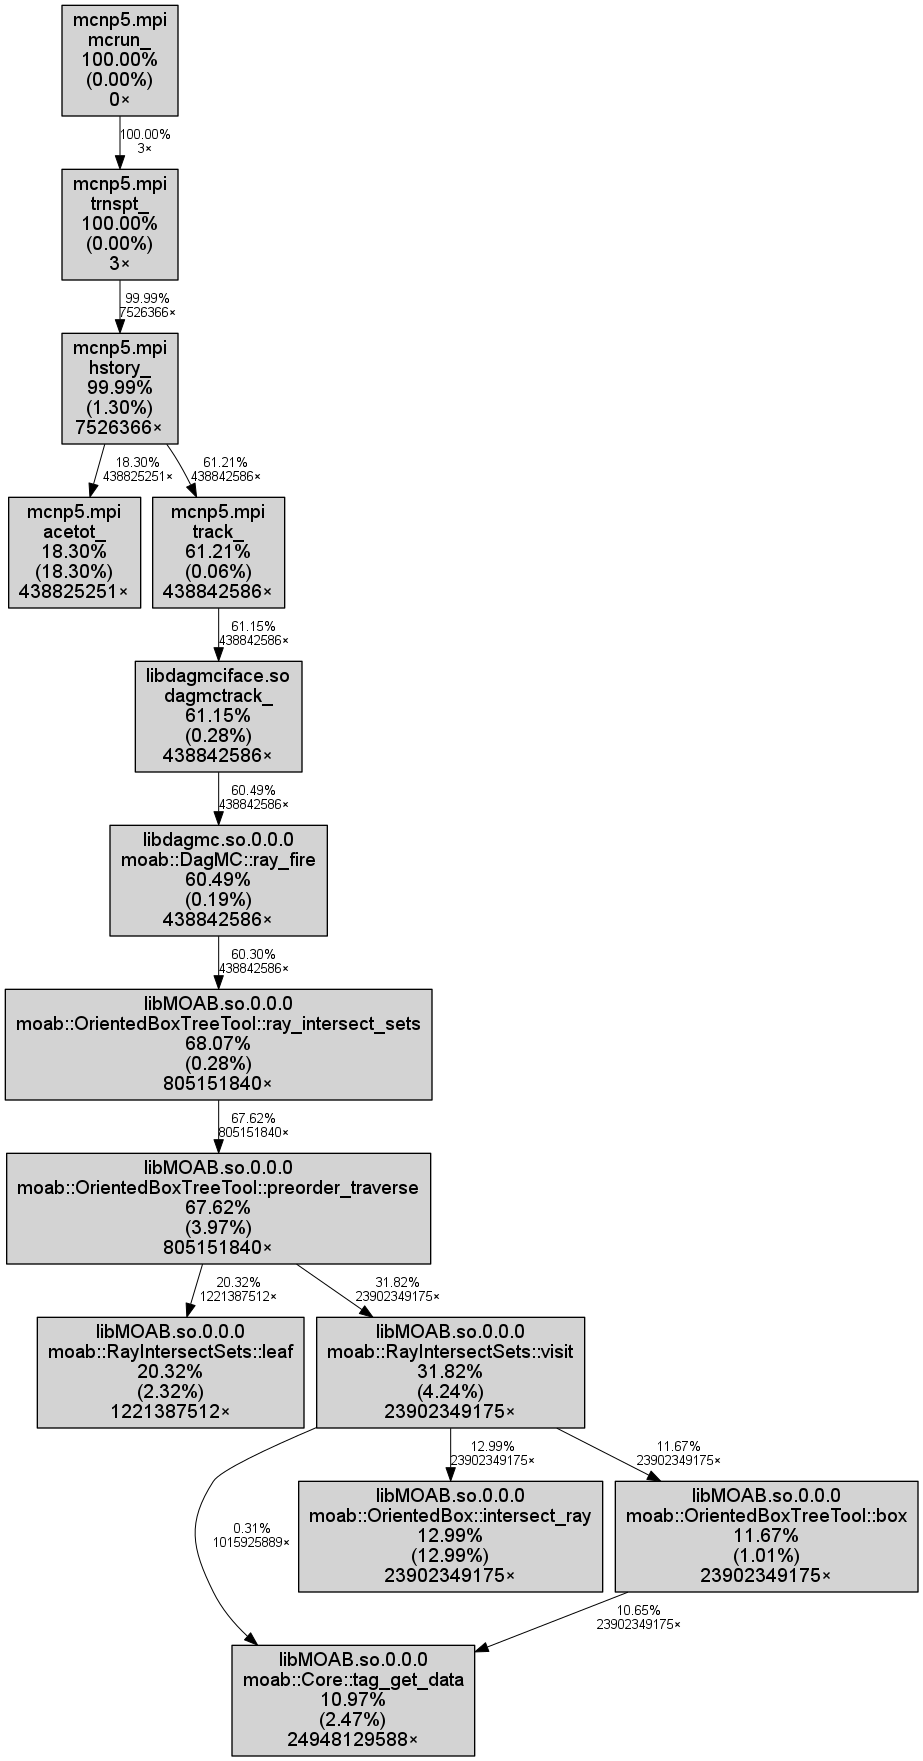
\includegraphics[scale=0.35]{dagmc_fng_cg_coarse.png}
\end{figure}

\begin{figure}[H]
  \centering
  \caption{Callgraph of native MCNP FNG run for 1E7 histories. (Processes taking $>$10\% of the runtime are filtered in order to simplify the call graph.)}
  \label{dagmc-fng-coarse}
  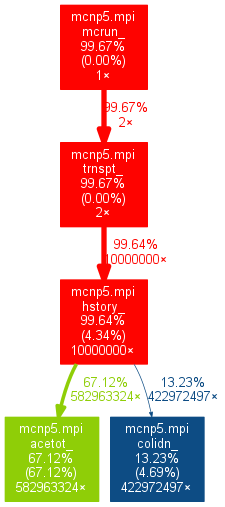
\includegraphics[scale=0.35]{mcnp_fng_cg_coarse.png}
\end{figure}

The combination of the profiling results indicating how much time is spent in tracking particles in DAGMC along with the difference in absolute run times confirms that indeed the performance bottleneck of DAGMC lies in its ability to quickly satisfy the geometric queries of the underlying Monte Carlo code it is coupled to. Looking more closely at the underlying calls in DAGMC, one can see that this time is collectively spent in the DAGMC ray\_fire call with the BVH traversal lying below this along with many underlying MOAB database-related calls. This indicates that this time is spent even more specifically in traversing MOAB's OBB BVH via the database-oriented methods available in DAGMC.

Again, it should be addressed that in this case a pre-built BVH was include in the geometry file and read into place much more quickly than in a typical DAGMC run. While this processes does contribute to additional DAGMC runtime, the amount of time spent building these hierarchies is small relative to the time spent in particle transport due to the high number of histories required for good statistics.


\section{High Valence Vertex Study}%%Status:In Progress%%
\label{hv_study}

One of the known bottlenecks of DAGMC is ray tracing performance degredation in regions with high-valence vertices. High valence vertices are defined as those connected to an unusally high number of triangle entities. This region of the mesh will take on a fan-like shape as seen in the figure below. High-valence vertices are known to occur on planar surfaces bounded by a circular curve. These regions are commonly generated in the faceting algorithms used to produce DAGMC meshes. This faceting scheme (which comes from ACIS libraries underlying the CUBIT/Trelis graphics engine) is designed to produce the smallest number of triangles possible to represent the model within the representation tolerance specified in DAGMC's surface mesh generation preprocessing step (dagmc\_preproc). Generally fewer triangles are better as even the ideal ray tracing acceleration structure queries for a given mesh scale as $O(log(N))$. However, even with fewer triangles undesirable configurations can impede performance as is shown by a set of tests conducted on models generated using this faceting scheme.

A study by Steve Jackson in 2011 on the performance of the MOAB ray tracer revealed a steep degredation in performance with a decreasing faceting tolerance and an increasing number of triangles. Using a DAGMC-based ray fire test program, the performance of DAGMC's ray fire ability was evaluated for four models. These models include a simple sphere, a notched sphere, a high aspect ratio cylinder, and an outer volume of an ITER model. In each of these tests, the models are tesselated with an increasingly smaller faceting tolerance in a higher number of triangles and more complex nature of the surface mesh in terms of BVH construction and traversal. The faceting tolerance being defined as the maximum distance between the faceted curve or surface and the geometric curve or surface which it resolves. 600k randomly oriented rays were then fired from the center of the volume isotropically.

\begin{figure}

  \begin{center}
    
    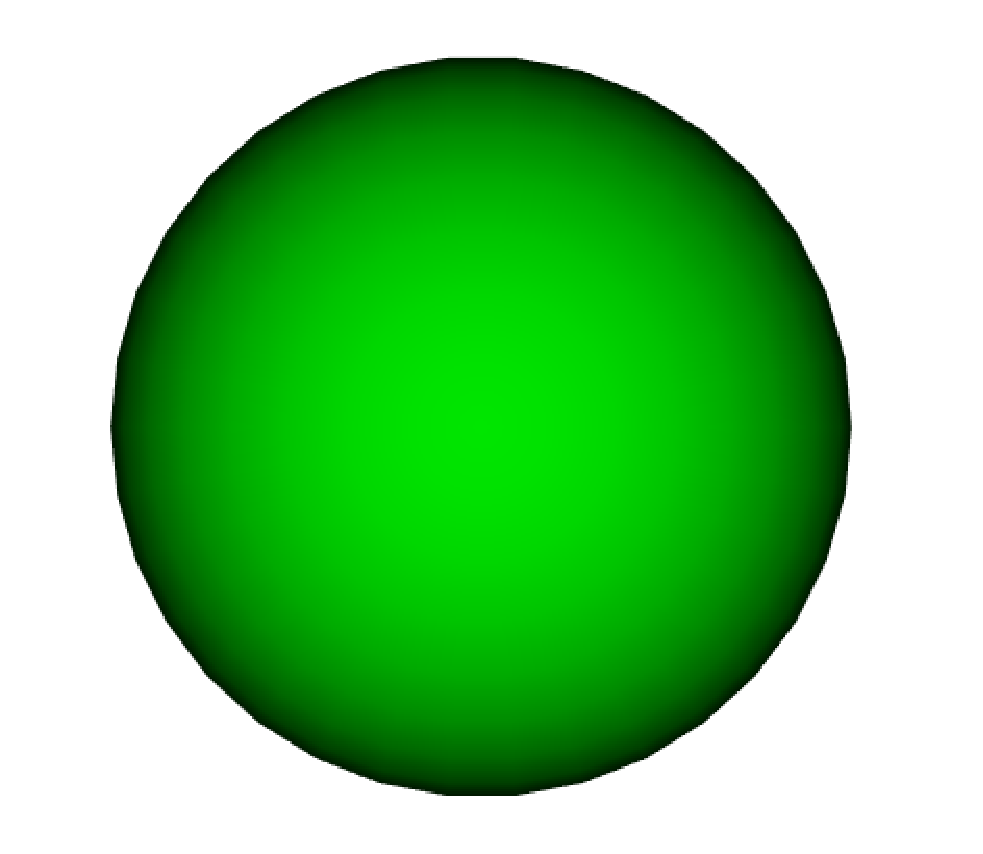
\includegraphics[scale=0.1]{sphere.png}
    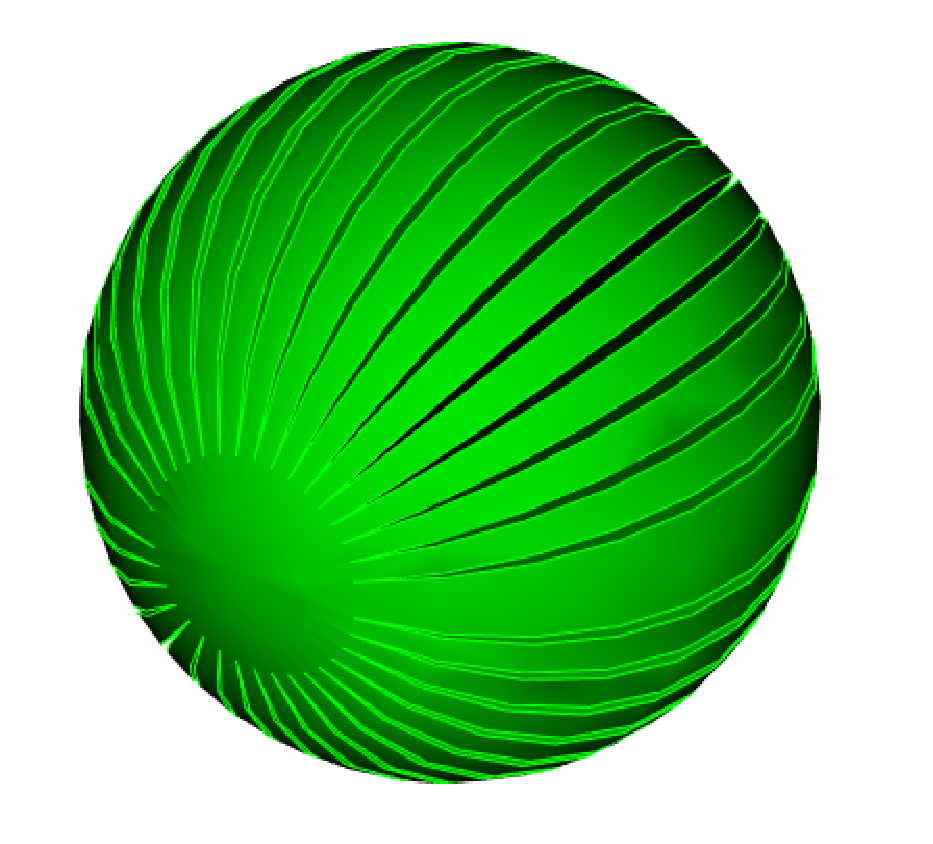
\includegraphics[scale=0.1]{ds.png}
    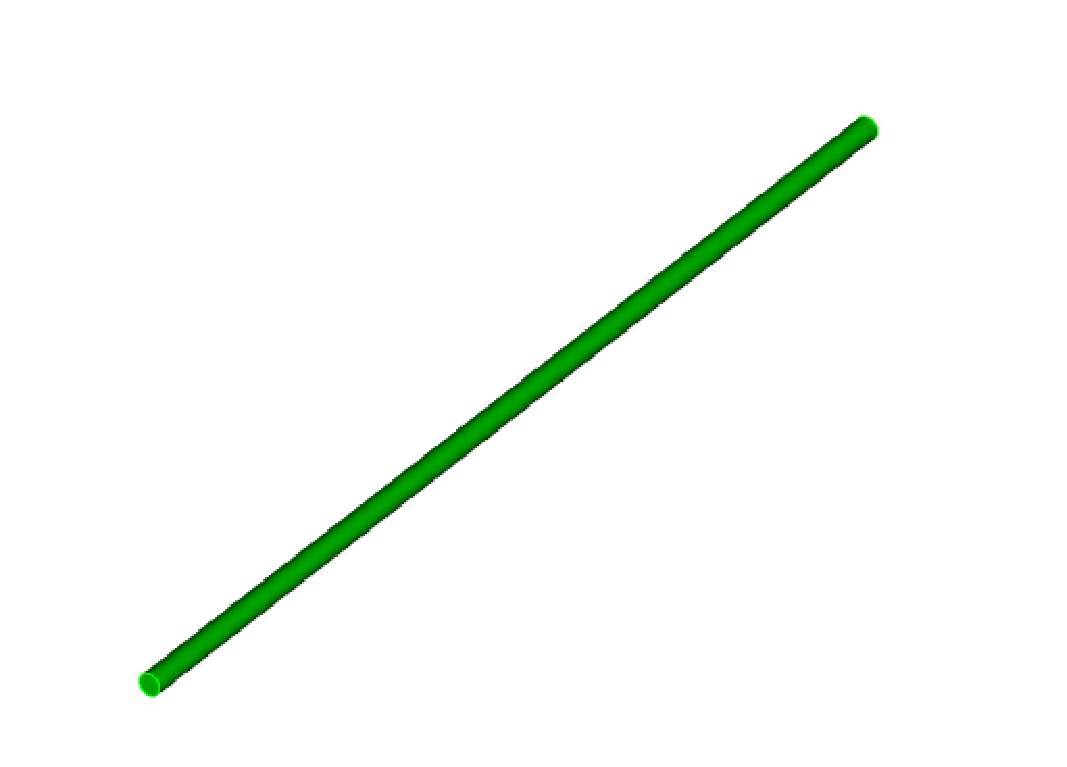
\includegraphics[scale=0.1]{larcyl.png}
    \caption{CAD representations of the sphere, slotted sphere, and high aspect ratio cylinder test models. (left to right) The ITER model is shown elsewhere. \label{models}}

  \end{center}
\vspace{-0.3cm}

\end{figure} 


Each model presents its own challenges with increasing faceting tolerance. The sphere is a good control case for an increasing number of triangles without change in complexity. The number of triangles generated in the spherical case will always increase with decreasing faceting tolerance, but the general nature of the triangulated surface (triangle density, structure, etc.) will remain the same. This is not true of geometries with planar surfaces which may be able to be resolved exactly using some finite number of triangles. In the case of the notched sphere, high-valence regions are generated by the faceting engine as a result of its underlying algorithms for planar surfaces meeting curves surfaces. The high triangle density of high valence regions cause overlaps in bounding volumes which become exacerbated as the faceting tolerance decreases. This results in inefficient hierarchy traversal. Additionaly, and perhaps more importantly than the presence of high valence regions, rays being fired with a point of origin at the center of the model causes them to travel either exactly along or very near to the surfaces of the planar slots in the sphere. Such a ray query will visit many internal nodes of the hierarchy during traversal, creating what is referred to as a very wide traversal as opposed to a narrow traversal in which fewer branches of the tree are explored. In this way, the slotted provides a good measure for the performance of a wide traversal through the hierarchy in a situation for which many of the internal nodes are required to be visited. The faceting of the high aspect ratio (HAR) cylinder contains many long, thin triangles running along the barrel of the cylinder. In similar fashion to the spherical model, the number of these triangles will increase with decreasing faceting tolerance resulting in an increasing triangle density as well. The low aspect ratio nature of these triangles can cause difficulty in the calculations of tightly fitting OBBs within MOAB's BVH builder. This test model is used to the ray tracing systems robustness of the BVH generation algorithms to objects with surface meshes of this nature. Finally, the faceting of a volume from an ITER model is used. This volume comes from a real world application of DAGMC's ray tracing kernel and is also known to contain high valence regions as well as seen in figure \ref{hv_examples}.

\textbf{Insert SJ tests here and disucss.}

- Insert origin SJ results
- Explain that terrible scaling was caused by the OBB bug
- Provide updated tests from MOAB with SJ's models
- Explain purpose of additional models
- Provide results with additional models
- Continue forward with test problems (already in place)
- Demonstrate ability to improve performance on the wedge model at the end of the section

In order to isolate the problem of high-valence vertices generated by the ACIS faceting algorithms, a new volume was added to the set of tests originally designed by Jackson in 2011.


\begin{figure}[H]
  \centering
    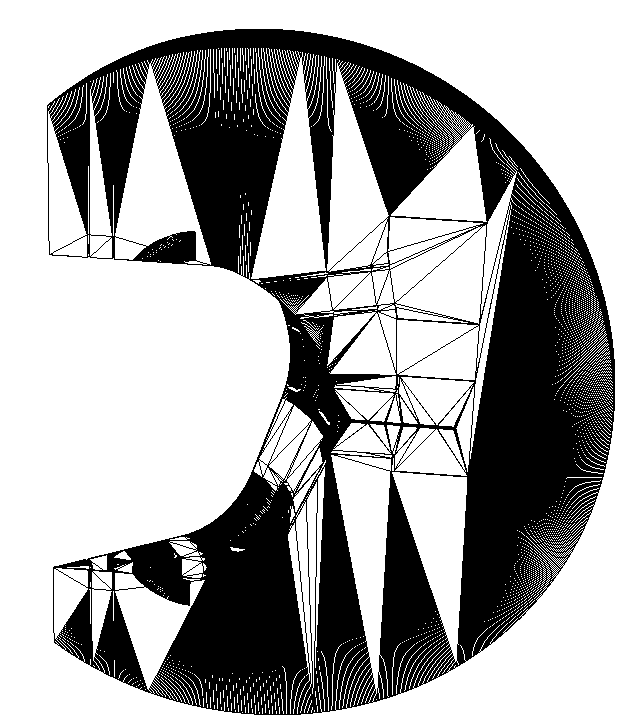
\includegraphics[scale=0.2]{iter_sideon.png}
    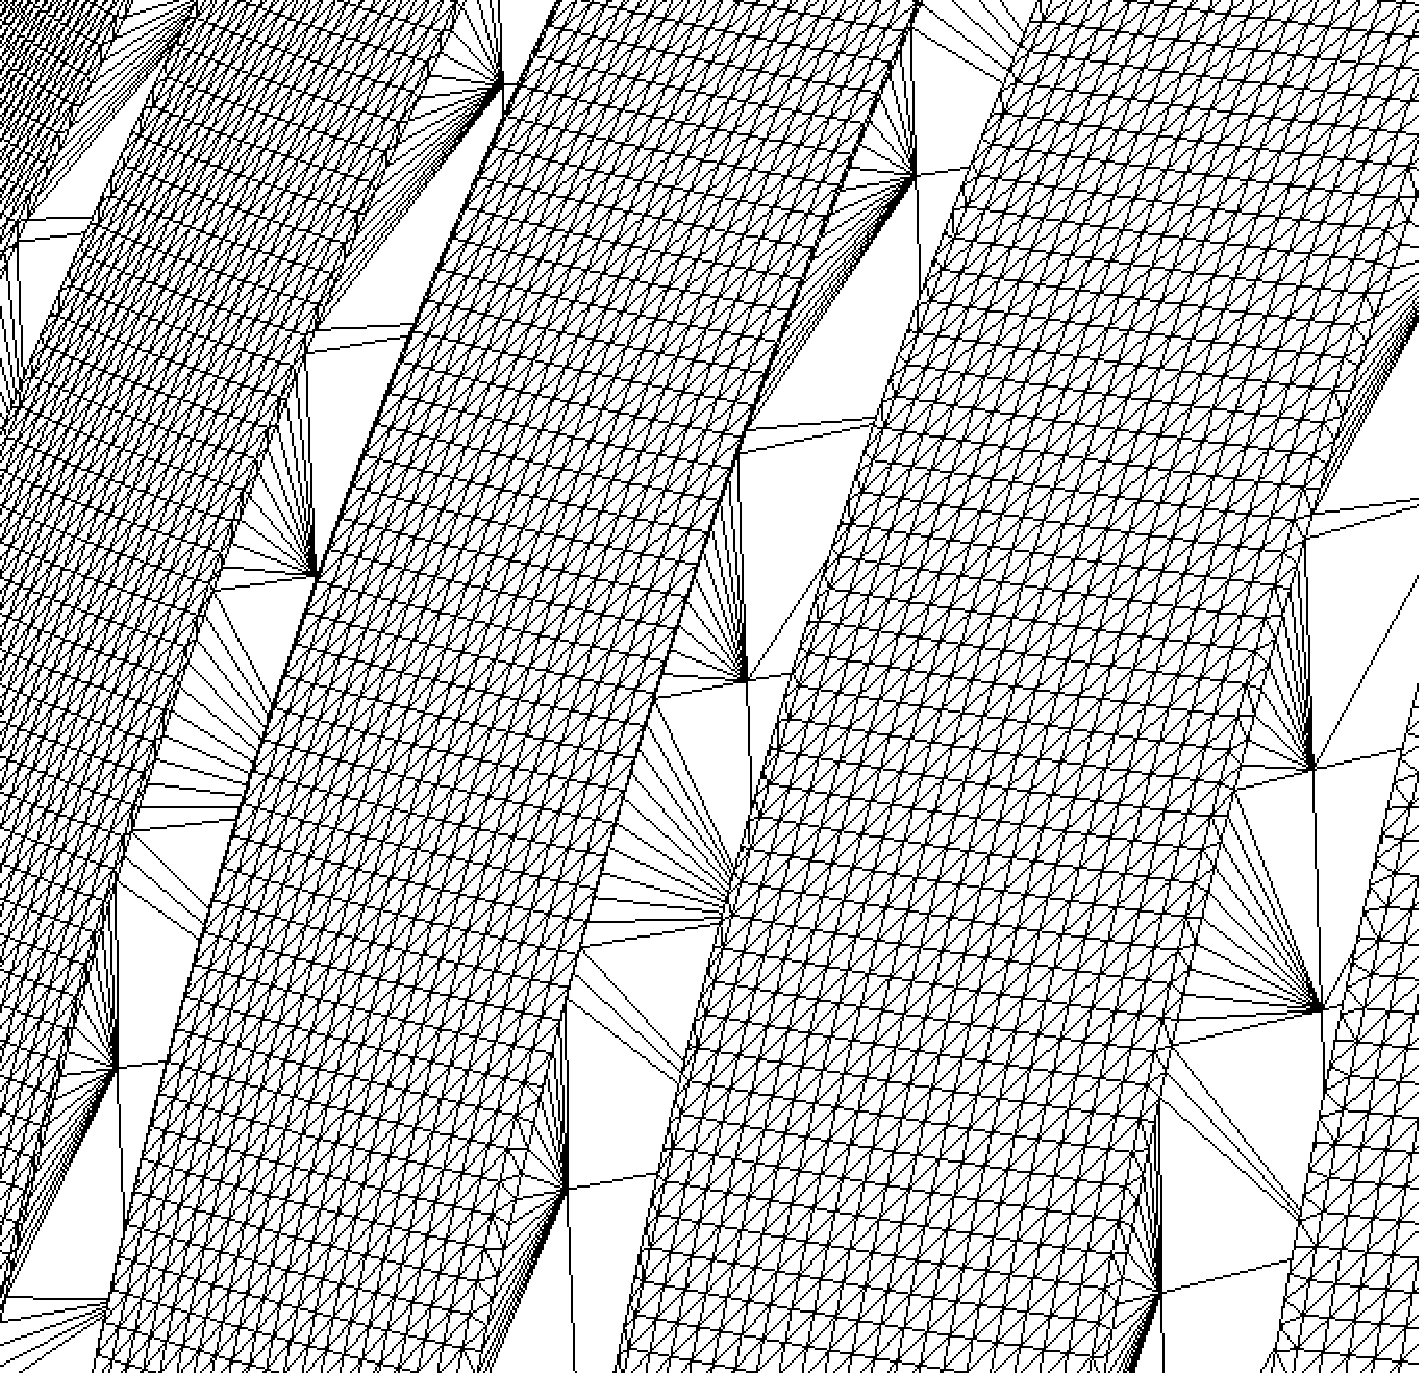
\includegraphics[scale=0.1]{ds_hv.png}
    \caption{Exampels of high valence regions in analysis and test models.}
    \label{hv_examples}
\end{figure}

To begin, a test mesh was manually generated in MOAB with an artificial high-valence region. This mesh is a modified cube centered on the origin in which the typical two-triangle faceting has been replaced by more complex planar surfce of triangles including an offset interior high-valence region within the face (please see figure below as a reference). The high-valence region was generated by inserting vertices along the diagonal of the interior box and connecting them to the opposing corners of the box. This effectively creates two adjacent high-valence regions, but this was necessary in order to maintain a watertight connectivity in the surface. This construction was designed such that the valence of the corner vertices in the interior region could be controled as well as the size of the interior region relative to the size of the entire face. Tests were then peformed on this model in order to characterize the performance impediment induced as well as its cause.

\begin{figure}[H]
  \centering
    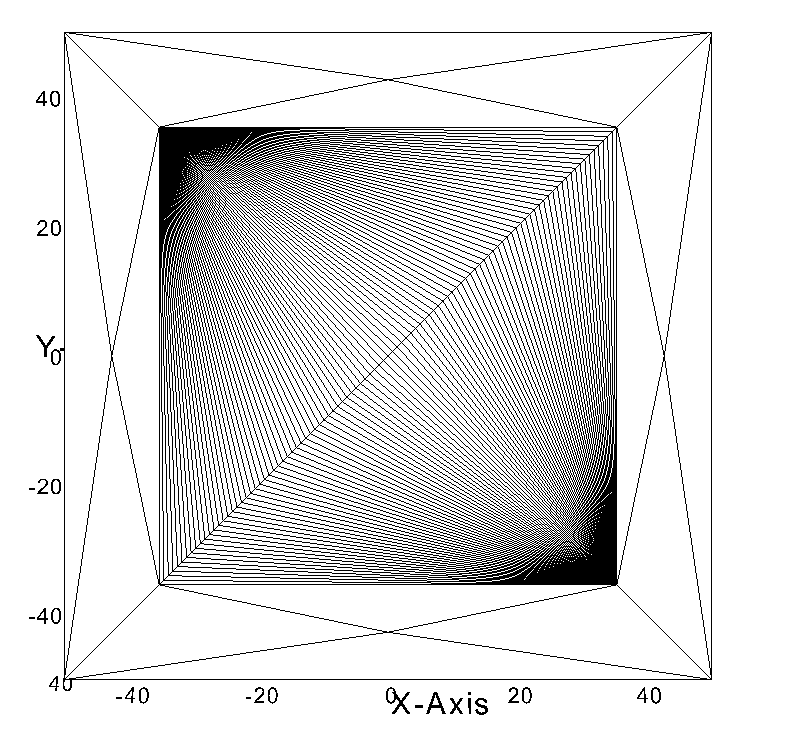
\includegraphics[scale=0.2]{hv_study_design.png}
    \caption{Side-on view of the modified cube mesh used to study the high-valence vertex problem.}
\end{figure}

A simple ray fire test program was used to construct ray tracing acceleration structures and conduct ray queries in DAGMC in the same way it would during particle transport. Information on this test program can be found in the appendix of this work. This program was used to fire rays with random direction from the origin of the test model while limiting the scope of the rays such that they should always find intersections on the modified surface containing the high-valence region. Many tests were done while varying the percentage of the surfce covered by the high-valence region as well as the valence of the region. Specification of the random number seed is allowed within the program, giving a more direct comparison of performance with the gaurantee that each test is firing the exact same set of rays.

All of the following tests vary the valence of the corner vertices from 2 to 50,000 and the fraction of the surface covered by the high valence region from 0 to 1. The following results come from DAGMC as it is being used now for all intensive purposes. From what is known about the nature of the BVH used in DAGMC, one would expect to see ray fire times increase as the area fraction increases (becuase rays are more likely to enter the high valence region) and as the valence increases (due to what we already know about its effect on the ray tracing speed). However, these results meet only one of those expectations. The ray fire times consistently become worse for an increase in valence, but for a given valence a lower area fraction actually shows a much longer ray fire time than the larger area fractions. This suggested that the presence of a high-valence region in a surface no matter the size could be causing problems in building and traversing the BVH. In order to investigate this matter further a visualization tool was developed to view the BVH as constructed by MOAB's building algorithm.

\begin{figure}[H]
  \centering
    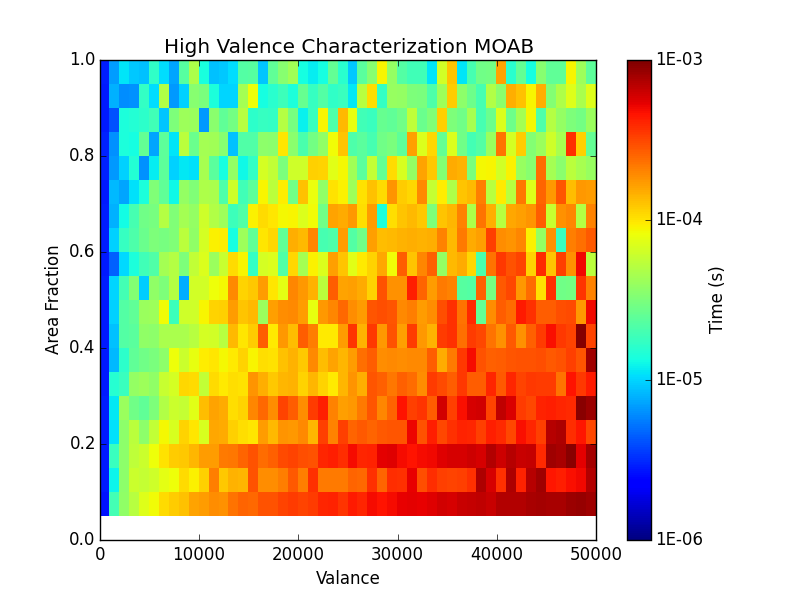
\includegraphics[scale=0.35]{hv_study_MOAB.png}
    \caption{Side-on view of the modified cube mesh used to study the high-valence vertex problem.}
    \label{hvsideon}
\end{figure}

Using a visitor pattern in the BVH, each oriented bounding box was converted into a MOAB hex element and saved on an different mesh instance. Each hex element was additionally tagged with it's depth in the tree as well as the triangle entities that it contains. This program then outputs a mesh which can be used to visualize the BVH level by level on top of the geometric mesh. At lower depths in the BVH, only bounding boxes in the high valence region are present. This is expected in that it will take more bounding boxes and therefore a deeper tree in that region in order to resolve the larger number of triangles. What was intereseting to note in this region was that the bounding boxes of the high valence surface would often contain some portion of the high valence region's triangles as well as other triangles in the high valence surface. Often bounding boxes like these would be leaf nodes of the tree (see below). Not only is this a problem in the sense that it implies a large number of triangle checks will be necessary if this leaf node is hit, but if this leaf node also contains triangles outside the high valence region with large area (as we tend to see in this model) the leaf becomes much more likely to be traversed, even though the chances that the ray is going to hit a triangle in the high valence region is relatively small. In this way the splitting algorithm not only deals with the high valence region poorly, but it may also create an artificially high probability of checking the high valence region's triangles if it contains other triangles in that retion.

\begin{figure}[H]
  \centering
    \includegraphics[scale=0.3]{{obbs_wsr_0.95}.png}
    \caption{View of culprit bounding box containing many high valence region triangle as well as other surface triangles.}
\end{figure}

MOAB's BVH building algorithm employs the median splitting method governed by a set of parameters use to determine if a node split is considered worthwhile by the building algorithm. One metric heavily favored by the algorithm is the splitting ratio of the resulting child boxes for a given splitting plane. The splitting ratio of a given node is defined by the absoulte difference in the entities between the child nodes divided by the total number of entities in the parent node. When building a BVH, MOAB sets a best and worst case value for this splitting ratio. If the splitting ratio for a given splitting plane is found to be better (smaller) than the best case splitting ratio then the node is split and the recursive top-down build continues. If the splitting ratio for a given splitting plane is worse than the worst case splitting ratio, then the node is not split. This is to avoid overly large/deep trees and large overlaps in sibling bounding boxes. If the splitting ratio is found to be between these two values, the ratio is tracked as further candidate split planes are tested. When all three median splitting planes have been checked, the child entity lists with the best splitting ratio is then used to perform the split.

In this case, the parameter of interest is the worst case splitting ratio. This parameter is intended to keep trees from becoming too deep by avoiding node splits which do not effectively divide entities. The default setting for the worst case split ratio is 0.95. In the case of the high valence vertices, many of the entities are packed tightly together, meaning that as the valency increases for a given area fraction, the splitting ratio will become worse and worse with splitting planes that are unlikely to divide these entities in a way that is seen as an acceptable split criterion by the building algorithm. Additionally, as the high valence region grows smaller relavitve to the surface size, this problem is only exacerbated in that the high valence region triangles become more closely packed together and less likely to be split by a median plane. The triangles exterior to the high valence region become larger relative to the area of high valence triangles contained by the node, causing the artificially high cross-section of the high valence region to be come larger as well.


  \begin{align*}
  splitting\;ratio  = \dfrac{|left\; child\; primitives\; -\; right\; child\; primitives|}{parent\; entities}
  \end{align*}

(mention triangle density shock in here maybe?)

  Fortunately MOAB allows one to have control over the parameters used to govern the BVH building algorithm. By altering this parameter, we can study its effect on the quality of the BVH and its adaptability to the high valence region. In addition to the valence and area fraction of the high valence region, the worst case split ratio was explored as well for values ranging between 0.95 and 1. The hypothesis here being that forcing the algorithm to continue splitting regardless of a poor splitting ratio on the number of entities would break up these prematurely ended branches in the BVH and eventually split up the high valence region as well.


  The test results for changes in this parameter show little change until the worst case splitting ratio reaches 1. This demonstrates the magnitude of the  perturbation the high valence region causes in the BVH building algorithm. However, when this parameter reaches t, the maxiumum value possible for the splitting ratio, the BVH builder is effectively forced to continue splitting until a new stopping criterion is met. This new stopping criterion is the minimum number of entities allowed in a single leaf. This value is based on an estimation of the number of ray-triangle intersection checks that can be done in the amount of time it takes to do a ray-box intersection check. Any more triangles than this in the leaf node and it would be more efficient to split the node. MOAB's BVH builder uses a default value of 8 for the minimum number of triangles allowed in a leaf node. The results of the same ray fire tests on the hv model using a worst case splitting ratio of 1 and an effective leaf criterion of a minimum number of entities are below.

  
\begin{figure}[H]
  \centering
    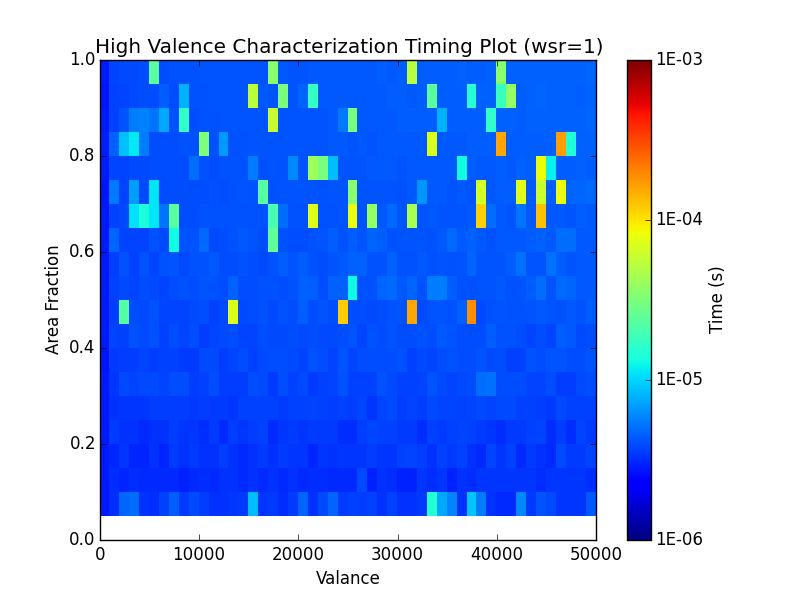
\includegraphics[scale=0.35]{hv_study_MOAB_wsr1.png}
    \caption{Rerun of the high valence characterization study with a worst case splitting ratio set to 1.}
\end{figure}


With this small change to the BVH builder's parameters, the timing of the high valence region becomes significantly better. This change is likely unsuitable for the general case of a tesselated surface however. A worst case splitting ratio of 1 would lead to much deeper trees which on average will take longer to traverse as well as consume much more memory for larger, more complicated models.

\section{Linking DAGMC with Intel's Embree}%%Status:In Progress%%
\label{emdag}

As mentioned in the previous section, a surprising number of MOAB-related database calls appear in the profiling of a DAGMC run. MOAB is a powerful tool for mesh generation, manipulation, and storage, but it was postulated that the implementation of a ray tracer in the context of this database design inherently comes with too much overhead for the implementation of an efficient ray tracer. As a result, an attempt at the replacement of MOAB's ray tracing system with a lean, highly-optimized ray tracer was made. Recently, Intel has made an effort to produce just such a CPU-based raytracer called Embree \cite{embree}. In both construction and traversal of BVHs, Embree takes advantage of many of the latest developments in BVH research at a programming level, and takes advantage of chipset architectures via vectorization at an implementation level. The combination of these effects leads to powerful raytracing tool in terms of performance. As a result of these factors and the effort that was put into producing Embree, it was chosen as the tool applied in DAGMC to satisfy geometric queries for MCNP. The resulting tool will be reffered to as EmDAG for the remainder of this discussion.

\subsection{Transferring DAGMC Model's to Embree Scenes}%%Status:Done%%

The process of employing Embree as DAGMC's ray tracer begins by establishing an equivalent representation of the MOAB mesh in Embree. In comparison to MOAB, Embree is limited in its ability to represent the underlying topological structure of a model. This topology is necessary and used advantageously during particle tracking in DAGMC by reducing the set of triangles queried to those of the particle's current volume. However, a way was discovered to represent enough of the topology to meet the requirements of DAGMC transport. The general representation of a model in Embree is referred to as a scene. Each scene may contain one or more geometries (meshes). Fortunately, this system is enough to create a workable representation of DAGMC meshes in which MOAB volumes are the equivalent of Embree scenes and MOAB surfaces are represented in their respective scenes as surfaces. This method provides a one-to-one mapping of MOAB volumes and surfaces to their corresponding entities in Embree and allows all topology-based operations to proceed inside of DAGMC in their usual manner. In this way, the requirement for topological information in DAGMC at the surface and volume level is met. Now transfer of the primitive mesh data can be considered.

Scenes do not share mesh data, so the triangle connectivity of each surface is reproduced in each scene they belong to. Fortunately, Embree does allow the sharing of vertices between scenes. In order to take advantage of this feature, all of the vertices in the MOAB mesh are provided in the Embree instance as a global vertex pool or buffer. Surfaces from all scenes can then be defined by a connectivity of vertices withing this pool. This method guarantees that the each surface can be represented by the same set of stored vertices in each scene it belongs to giving the exact same representation in each scene. It greatly simplifies particle tracking by guaranteeing that the same topological surfaces will not overlap each other in different scenes and will maintain watertightnes at the boundaries between surfaces.

The representation of triangle normals are important to the DAGMC particle tracking algorithm established by Smith et. al. \cite{smith_thesis_2011} in 2011. In DAGMC, particles on or just outside the surface of a volume are handled by ignoring the near-surface intersection upon being established in a new volume. This is accomplished using the convention that triangle normals will always point outward from the center of the volume they belong to. Triangles hit by the ray are ignored if the normal of the triangle opposes the ray direction via a dot product calculation. While this has historically been handled inside of DAGMC, this is accomplished in EmDAG via the use of Embree's filter functions. Filter functions allow for a user-defined callback method which allows users to validate a ray hit inside of Embree before returning a final result. Embree will return is most recent intersection with the scene to the filter function (the hit triangle's unnormalized vector included) and allow a method to either accept the hit or instruct Embree to continute tracing the ray path based on the outcome of the filter function. In MOAB, triangle normals are set in a global manner and adjusted using stored information within MOAB based on what volume is being queried at the time. This is referred to as the surface's sense with respect to that volume. Because we are forced to duplicate surfaces in Embree, the triangle normals are pre-oriented based on this surface's sense for the scene it is being created in upon initialization of the model within the Embree instance. This saves steps in gathering this information upon traversal when the triangle normal is needed to determine a particle's logical position within the model. The resulting memory footprint of EmDAG after duplicating the DAGMC geometry in Embree is not much greater thanks to the single precision values used in Embree. The single nature precision of Embree and its effect on DAGMC will be discuseed further in later sections of this work.
By meeting these requirements of topology, watertight representation, and hit acceptance/rejection based on triangle normals, Embree provides DagMC with all the information needed to perform geometric operations required by the various Monte Carlo codes it supports, but in an agnostic manner to the ray tracing kernel being used.

\subsection{EmDAG Performance and Testing}%%Status:In Progress%%

Using the same DAGMC-based ray fire test program, the performance of DAGMC's ray fire ability was compared to that of EmDAG's for three models. These models include a simple sphere, a notched sphere, and a high aspect ratio cylinder. In each of these tests, the models are tesselated with an increasingly smaller faceting tolerance in a higher number of triangles and more complex nature of the surface mesh in terms of BVH construction and traversal. The faceting tolerance is defined as the maximum distance between the faceted curve or surface and the geometric curve or surface which it resolves. 600k rays are then fired from the center of the volume isotropically using the same random number seed so that the same set of rays is fired in each ray tracing system.

\begin{figure}

  \begin{center}
    
    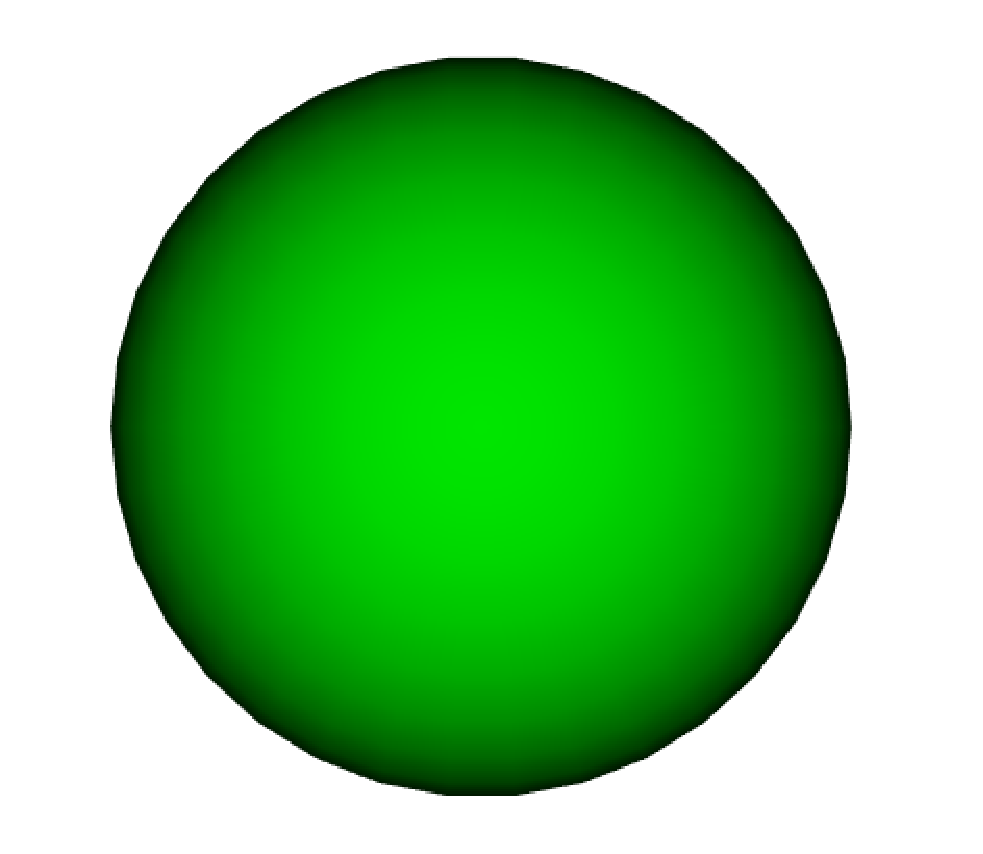
\includegraphics[scale=0.1]{sphere.png}
    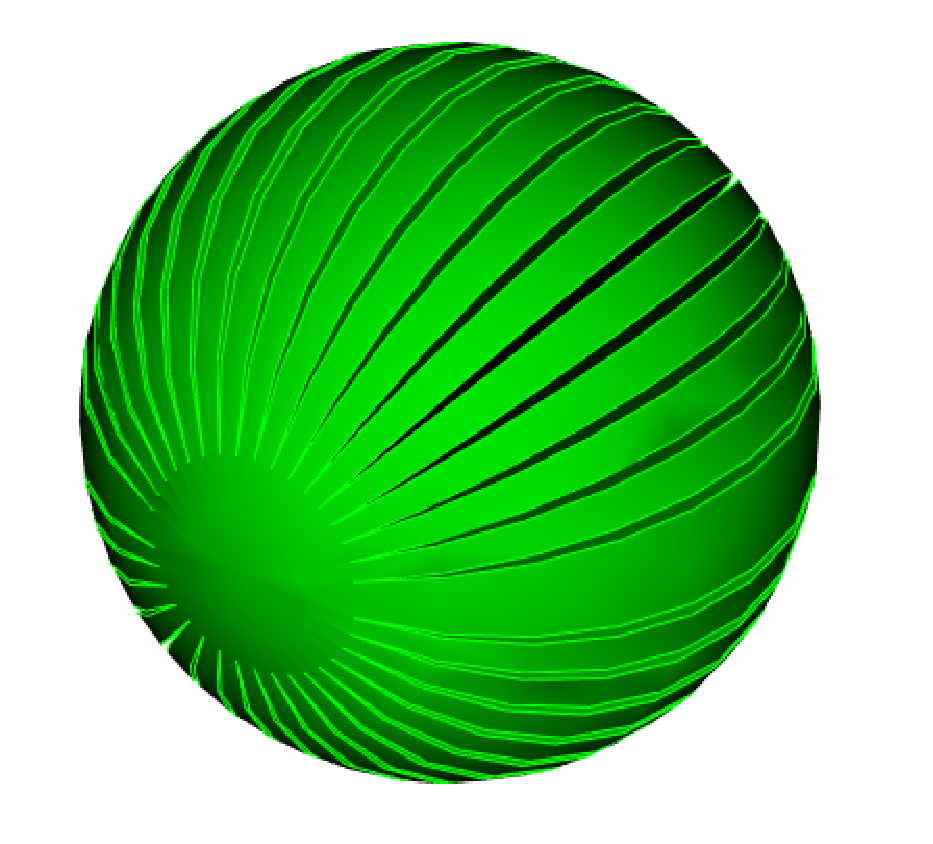
\includegraphics[scale=0.1]{ds.png}
    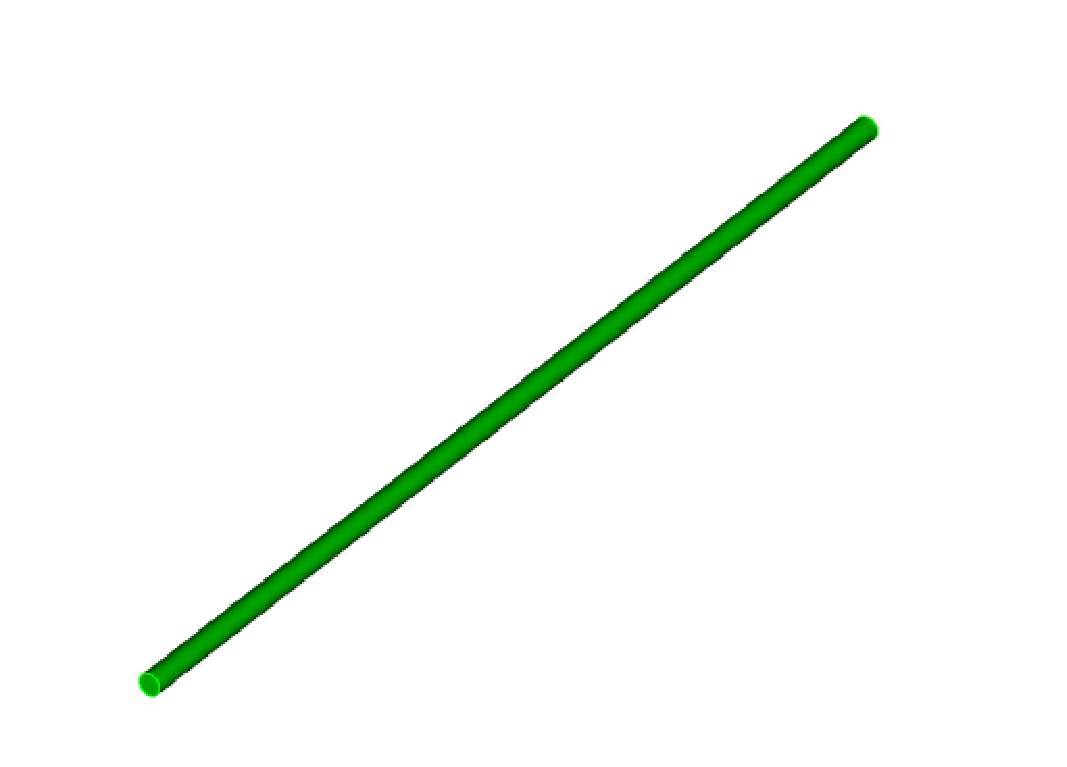
\includegraphics[scale=0.1]{larcyl.png}
    \caption{CAD representations of the sphere, slotted sphere, and high aspect ratio cylinder test models used for ray fire timings of DagMC and EmDagMC. (left to right) \label{models}}

  \end{center}
\vspace{-0.3cm}

\end{figure} 


Each model presents its own challenges with increasing faceting tolerance. The sphere is a good control case for an increasing number of triangles without change in complexity. The number of triangles generated in the spherical case will always increase with decreasing faceting tolerance, but the general nature of the triangulated surface (triangle density, structure, etc.) will remain the same. This is not true of geometries with planar surfaces which may be able to be resolved exactly using some finite number of triangles. In the case of the notched sphere, regions referred to as ``high valence'' are generated by the faceting engine as a result of its underlying algorithms for planar surfaces meeting curves surfaces. High valence regions are defined by an area in which a single vertex is connected to an abnormally high number of triangles and will be discussed in detail later. High valence regions are a difficult problem for many BVH building algorithms. The high triangle density of high valence regions cause overlaps in bounding volumes which become exacerbated as the faceting tolerance decreases resulting in inefficient hierarchy traversal. The faceting of the high aspect ratio (HAR) cylinder contains many long, thin triangles running along the barrel of the cylinder. In similar fashion to the spherical model, the number of these triangles will increase with decreasing faceting tolerance resulting in an increasing triangle density as well. The low aspect ratio nature of these triangles can cause difficulty in the calculations of tightly fitting OBBs within MOAB's BVH builder. This test model is used to the ray tracing systems robustness of the BVH generation algorithms to objects with surface meshes of this nature.

The standard DAGMC ray fire test program (included in appendix A) was used to evaluate both ray fire systems. The test program itself is agnostic to the underlying ray tracing kernel used by DAGMC and two versions of the program were compiled. One in which DAGMC uses MOAB's ray tracer and another in which MOAB's ray tracing system is subverted by Embree, a.k.a. EmDAG. The two sets of timing results can be found side-by-side below.

\begin{figure}
  \centering
  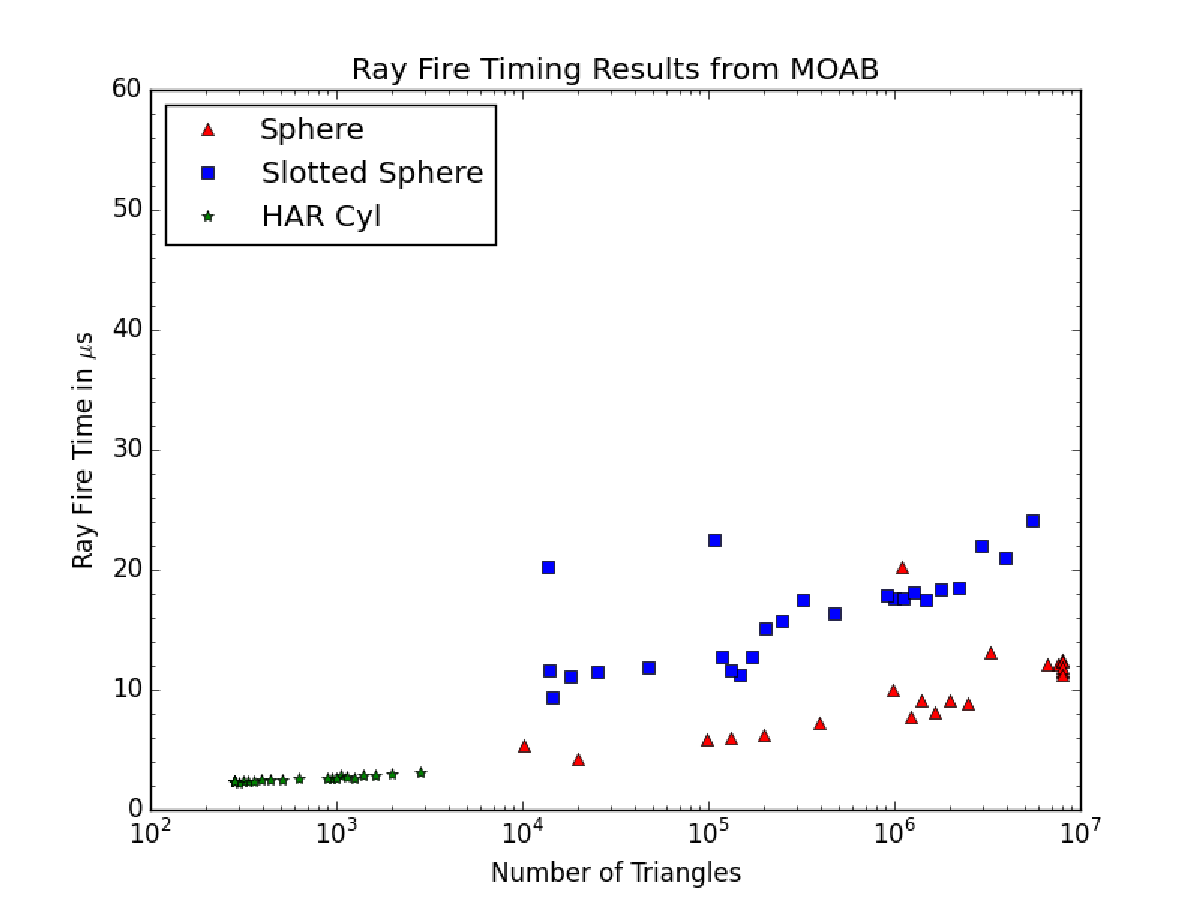
\includegraphics[scale=0.2]{Eig_fix_rf.png}
  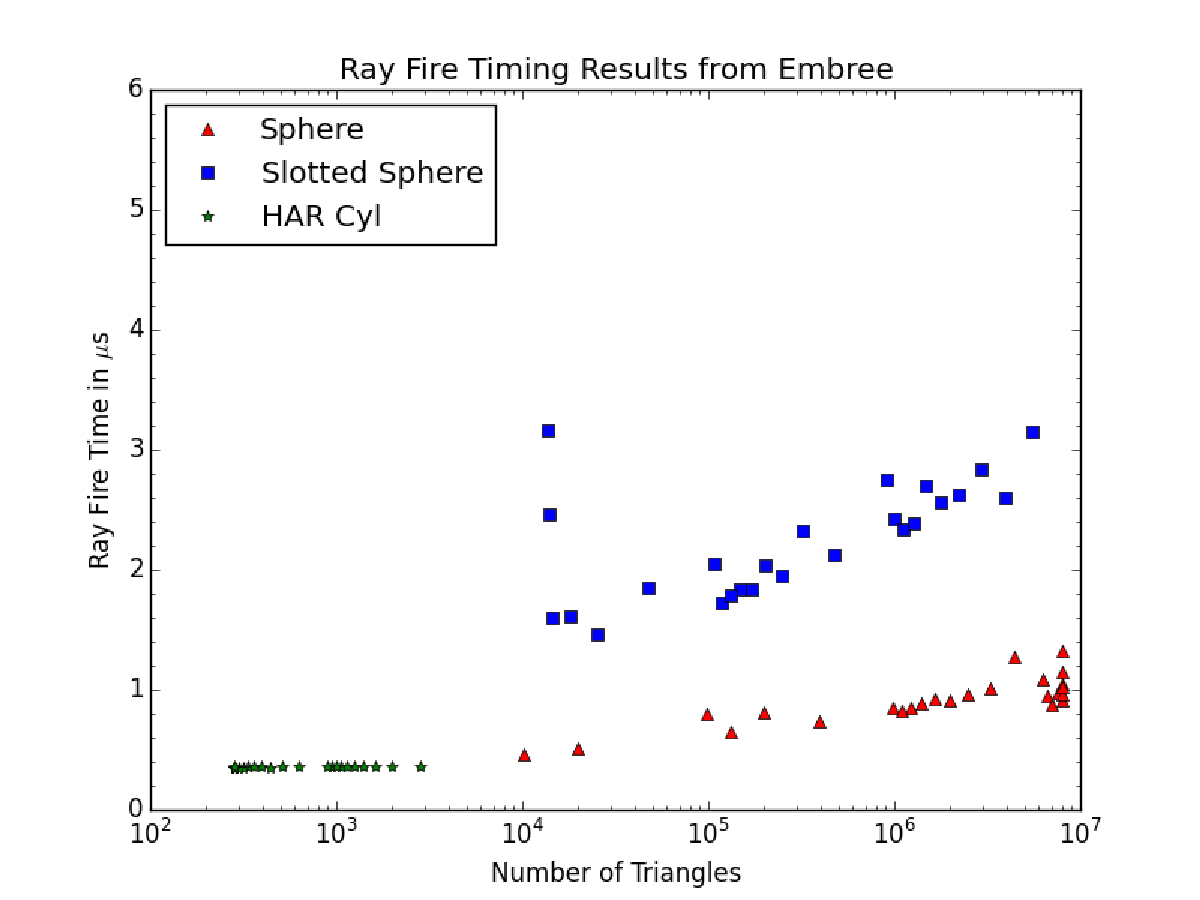
\includegraphics[scale=0.2]{embree_rf.png}
  \caption{A comparison of ray fire times between DAGMC using MOAB's ray tracing and Embree. Please note the difference in time scale.}
\end{figure}

The results of these tests validate the suspicion that the MOAB database contains a considerable amount of overhead for the implementation of a ray tracing kernel. This is indicated in the way that the ray tracing times scale for each model in both kernels. From a faceting tolerance scaling point of view, both systems scale relatively well for the HAR cylinder. This indicates that both systems are capable of building bounding volumes robustly for a model with long, skinny triangles. The scaling of the spherical case is slightly worse off than the HAR cylinder most likely because the BVH tree is going to becomce gradually deeper as more and more triangles exist in the model needing to be resolved by the BVH. Finally, the slotted sphere contains many high valence regions and as expected it scales the worst with decreasing faceting tolerance as the valency of these regions increases. It is very apparent that there is nearly an order of magnitude difference in the ray fire timings MOAB and Embree. Due to the very similary scaling of each test model, it can be stated that the majority of the descrepancy in the ray fire timings between the two systems occurs in the traversal methods employed by both systems and isn't likely due to a large advantage in the structure of the BVH being built by either system. Changes in the way the BVH is built typically accounts for anywhere from 30-40\% difference in ray fire timings whereas the descrepancy seen here between MOAB and Embree is on average \textbf{an order of magnitude better} using Embree. In large part, this has to do with Embree's freedom of design without the restriction of a ray tracing implementation inside the context of another application. It should be addressed that the vectorization of Embree's traversal also contributes greatly to its speed relative to MOAB. This can be also considered a part of the design freedom allowed when designing an independent ray tracing system that could not be afforded using MOAB's database practices as well. However, a property unique to MOAB in the world of mesh tools may allow for an implementation such as this as will be discussed near the end of this work.

As an extension of these pure ray fire tests, the effect of an improved ray tracing system on particle transport was studied as well. These tests begin with several simple models and end with the application of EmDAG to one of the performance benchmark modles - the Frascati Neutron Generator model. The first transport models to be tested were a single cube and single sphere filled with a dense hydrogen material for high collisionality in the problem. Each of these models' principal dimension is 10 cm. The source for these models is a 5 MeV neutron isotropic point source at the center of the volume and 1 million particles were run in each test. All of the test models were preproccessed using a faceting tolerance of 1e-04. Moving upward in complexity, another set of tests were run using a set of nested cubes and nested spheres. Each of the nested volume models contained three cells: the inner volume, a shell volume, and the graveyard volume. The purpose of these tests was to ensure that particles could in fact be tracked through multiple volumes. The nested cubes model contains an extra volume which consists of the original single cube subtracted from a cube 1cm larger in each dimension. The nested sphere model contains an extra volume consisting of the original sphere from the single volume model subtracted from a sphere 1cm larger in radius. As the purpose of these tests was to test EmDAG's particle tracking between non-zero importance cells, the dimensions of the offset between the nested volumes is largely irrelevant so long as particles are in fact reaching all of the cells.

\begin{table}[H]
  \small
  \begin{center}

      \label{timings}
    \begin{tabular}{lccc}

      \toprule
      Test Model & MCNP & DagMCNP & EmDagMCNP \\
      %%\hline
      & \multicolumn{3}{c}{\textbf{time (min)}} \\
      \hline
      Sphere & 2.93 & 25.13 & 4.73  \\
      Cube & 5.03 & 10.56  & 5.80 \\
      Nested Spheres & 4.35 & 50.82 & 7.94 \\
      Nested Cubes & 4.73 & 9.26 & 4.35 \\
      %%\hline
      &  \multicolumn{3}{c}{\textbf{histories/min}} \\
      \hline
      Sphere & 3.4104E+05  & 3.9944E+04  & 2.1810E+05   \\
      Cube & 1.9879E+05 & 9.4738E+04 & 1.7260E+05 \\
      Nested Spheres & 2.2991E+05 & 1.9877E+04 & 1.3947E+05 \\
      Nested Cubes & 2.1170E+05 & 1.0806E+05 & 2.3026E+05 \\
      \bottomrule
      
    \end{tabular}
  \end{center}
  \caption{Runtime comparison native MCNP, DAG-MCNP, and EmDAG-MCNP for four identical test problems.}
  
\end{table}

The native MCNP runs were generally the fastest among the test problems with the exception of the nested cubes case in which EmDAG-MCNP marginally outperformed the native code by ~8\%. This is likely due to the fact that very few triangles are needed to exactly represent the surfaces of cubic volumes. This creates a very simple problem in the area of BVH building and results in a very shallow tree. The fact that these volumes have many surfaces is also of importance here. MCNP searches linearly through a given cell's (volume's) surfaces to determine the intersection of a particle with the nearest surface whereas both DAG-MCNP and EmDAG-MCNP perform this search spatially. In the nested cubes model, it is likely that the number of surfaces relative to the number of triangles in their representation is high enough to allow EmDAG-MCNP to overtake MCNP's CSG calculations. 




\begin{table}[H]
  \small
  \begin{center}
    \caption{Nested Spheres Tally Results. Flux tally units are $cm^{-2}$. Energy tally units are MeV/g. Note: result comparisons of other test cases can be found in Appendix B.}
    \label{nestedspheres}
    \begin{tabular}{lccc}
      \toprule
      Value & MCNP & DagMCNP & EmDagMCNP \\
      \toprule
      %%Hist/min & 2.2991E+05 & 1.9877E+04 & 1.3947E+05 \\
      %%\hline
      \multicolumn{4}{l}{\textbf{Cell 1 Tallies}} \\
      \hline
      Flux  & 5.25725E-03 & 5.25734E-03 & 5.25734E-03 \\
      Energy  & 3.17869E-03 &  3.17873E-03 &  3.17873E-03 \\
      \hline
      \multicolumn{4}{l}{\textbf{Cell 2 Tallies}} \\
      \hline
      Flux  & 1.91645E-04 & 1.91644E-04 & 1.91644E-04 \\
      Energy  & 5.22131E-05 & 5.22137E-05 & 5.22137E-05 \\
      \hline
      \multicolumn{4}{l}{\textbf{Cell 3 Tallies}} \\
      \hline
      Flux  & 1.18371E-05 & 1.18376E-05 & 1.18410E-05 \\
      Energy  & 4.96282E-06 & 4.96285E-06 & 4.96285E-06 \\
      \bottomrule
                        
    \end{tabular}

  \end{center}
%%\vspace{-0.2cm}
\end{table}


The results of the single-volume test cases for native MCNP differ slightly from the agreeing tally results from the DAGMC-based systems. This is not surprising as DAGMC is known to report slightly different results from native MCNP and this was not necessarily the concern of this study. However, differences in the tally results between DAG-MCNP and EmDAG-MCNP are present in the nested spheres model. This results in a small difference in the flux tally for cell 3 as can be seen in Table \ref{nestedspheres}. By examining the number of particle tracks in each cell, it can be determined that this discrepancy is caused by a single particle ending in EmDAG-MCNP near a surface of cell 2 while in DAG-MCNP the particle crosses into cell 3 before abruptly dying though it still contributes slightly to the tally in that cell. It is believed that this difference in tally result is the result of a systematic difference between Embree and MOAB's ray fire conventionality rather than Embree's a result of the double to single floating point conversion of the model that occurs when using EmDAG.

Finally, a full-scale test of EmDAG was conducted on the FNG model using the same volumetric source as in the performance benchmarking tests described earlier. Initially this model failed quickly due to lost particles. This was surprising as the model is expected to have the same watertight fidelity that it does when using DAGMC. In order to allow the run to complete, the number of allowed lost particles was increased to the number of the sources particles being run (1e8). The justification for this allowance being that if the lost particle rate is small enough, overall performace and results of the run would still provide a viable comparison of the two systems. In the end, the model lost 255 particles in 1e8 histories. This rate isn't expected to change the perfomance or result of the overall run in a significant way. A comparison of the FNG run using EmDAG-MCNP to the native MCNP model as well as DAG-MCNP is found in Table \ref{fngemdag}.


\begin{table}[H]
  \small
  \begin{center}
    \caption{Nested Spheres Tally Results. Flux tally units are $cm^{-2}$. Energy tally units are MeV/g.}
    \label{fngemdag}
        \begin{tabular}{|c|c|c|c|c|}
      \hline
      \textbf{Implementation} & \textbf{ctme (min)} & \textbf{wall time (min)} & \textbf{lost} & \textbf{ratio} \\
      \hline
      MCNP5 & 209.92 & 205.99 & 0 & 1.00 \\
      \hline
      DAG-MCNP5 & 1023.04 & 1023.05 & 0 & 4.99 \\
      \hline
      EmDAG-MCNP5 & 303.49 & 303.63 & 255 & 1.44 \\
      \hline
      EmDAG-MCNP5 (lt) & 257.49 & 257.60 & 247 & 1.25 \\
      \hline
    \end{tabular} 

  \end{center}
%%\vspace{-0.2cm}
\end{table}


\begin{figure}
  \centering
  \caption{Callgraph of the EmDAG run on the FNG model for 1E7 histories. (Processes taking $>=$6\% of the runtime are filtered in order to siplify the callgraph.}
  \label{emdag-fng-coarse}
  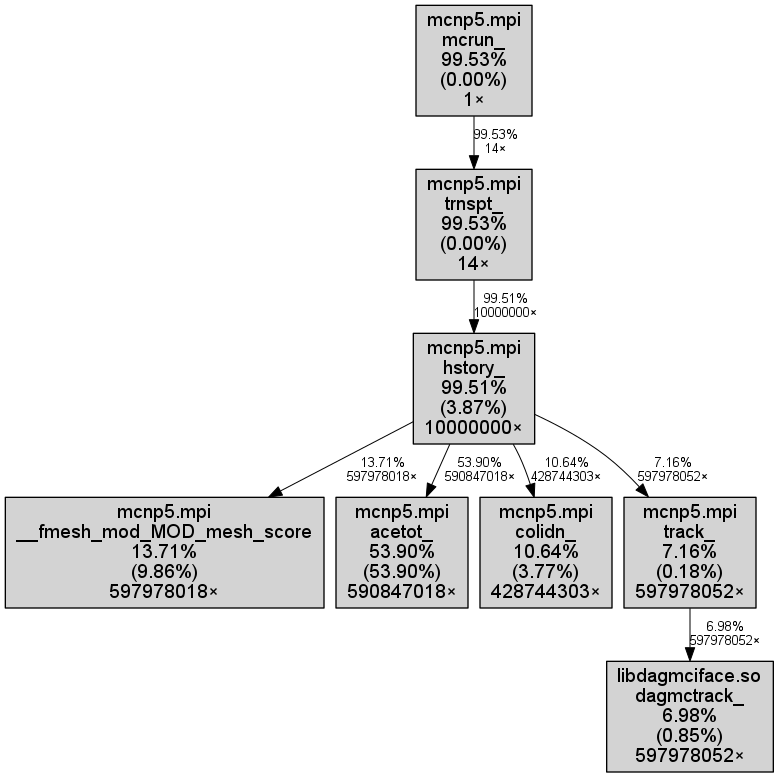
\includegraphics[scale=0.35]{emdag_fng_cg_fine6.png}
  
\end{figure}




While the performance of EmDAG greatly surpases that of DAGMC, it does not come as close to the performance of native MCNP as it did in the case of the test models. Upon visually inspecting the faceted FNG model, it was seen to contain many high valence regions. As an artifact of the variance reduction used in the intended analysis of this model, many planes were inserted in the model in order to break up large cells with highly varying particle intensities. Where these planes intersect the cylindrical volumes of the model, many high valence regions result as can be seen in figure \ref{fng-faceted-models}. As a result it became a curiousity as to whether or not the high valence regions were being handled better by EmDAG than they were by DAGMC. In order to test this, the same programs used to do the high valence vertex study were built using EmDAG and the parameter sweep of the relative high valence area and valency were run. The results in figure \ref{emdaghvstudy} show that EmDAG does in fact struggle these high valence regions. In the worst scenario we see a degradation by two orders of magnitude compared to the best case scenario which is similar to what was seen in the unmodified MOAB ray tracer. Additionally, it shows degraded performance in the same way that DAGMC was initally expected to falter - with increasing high valence area and valency. This is likely due to the nature of the heuristics used by Embree to construct its acceleration datastuctures. Embree employs the surface area heuristic in building its BVH which may have something to do with this performance issue. Unlike MOAB, however, the option of altering the BVH building parameters is not availble to us. There is, however, an option to reduce the size of the high valence regions in the mode within the faceting algorithm by definig a length tolerance. The length tolerance is a maximum length for any faceting edge returned by the faceting algorithm. Defining this value comes at the cost of many more triangles than needed to define a model within some faceting tolerance which gives a more clear definition of the model's fidelity relative to the analytical underlying representation of the geometry. The difference in facet structure between these models can also be seen in figure \ref{fng-faceted-models}. By generating a faceted model using the combination of the length and faceting tolerances it was hoped that there would be a marked increase in performance using the EmDAG system and the performance did indeed improve by ~15\%. Due to the increased number of overall triangles on these planar surfaces, there may be competing forces at play. As the length tolerance is reduced, the high valence areas will also be reduced, but the overall number of triangles will increase resulting in inherently deeper BVH and longer traversals. Conversely as the length tolerance is increased, the high valence areas are increased as a result, but the number of redundant triangles is reduced perhaps improving the average BVH traversal time enough compensate for a few more rays entering high valence regions as a result of their incresed area. The length tolerance of the FNG model could then be optimized. This optimization study, while interesting, will vary model to model and the results will be complex in nature, depending on the underlying geometry and geometry adjacent to those regions, etc. In light of the high valence study results showing that BVH building parameters can be altered to improve performance and accomodate these high valence regions, it seems a better, and simpler answer over alteration of the mesh globally in the model. Nonetheless, while it may be possible to alter the building parameters of Embree as was done wit MOAB, but an interface for this does not currently exist within the Embree API and would likely require large alterations to code to allow access such as that. Given these truths, in order to determine how close the current EmDAG system could come to native MCNP performance on the FNG model with the tools available a number of length tolerances were tried when faceting the FNG model.  

\begin{figure}[H]
  \begin{center}
    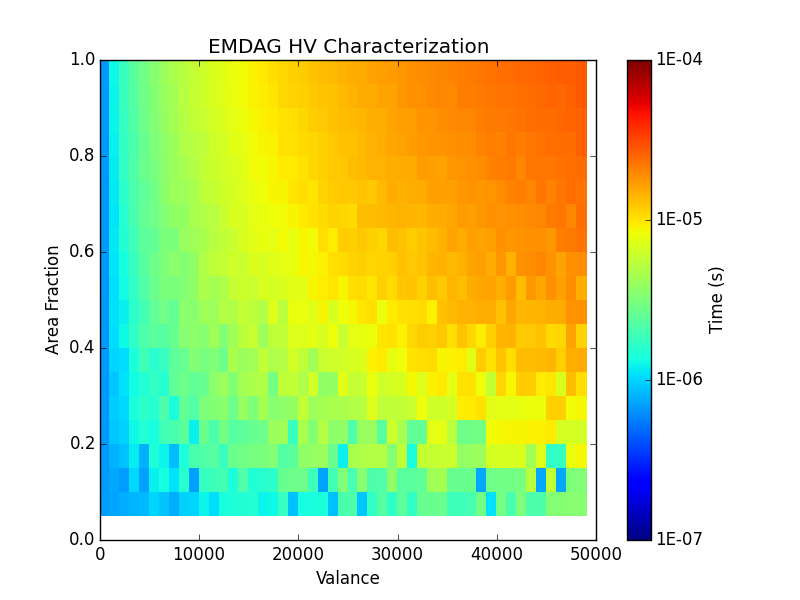
\includegraphics[scale=0.35]{hv_emdag.png}
    \caption{High valance study results using EmDAG. Please note the alterations to colorbar limits made to use color scale effectively.}
    \label{emdaghvstudy}
  \end{center}
\end{figure}

\begin{figure}[H]
  \small
  \begin{center}
    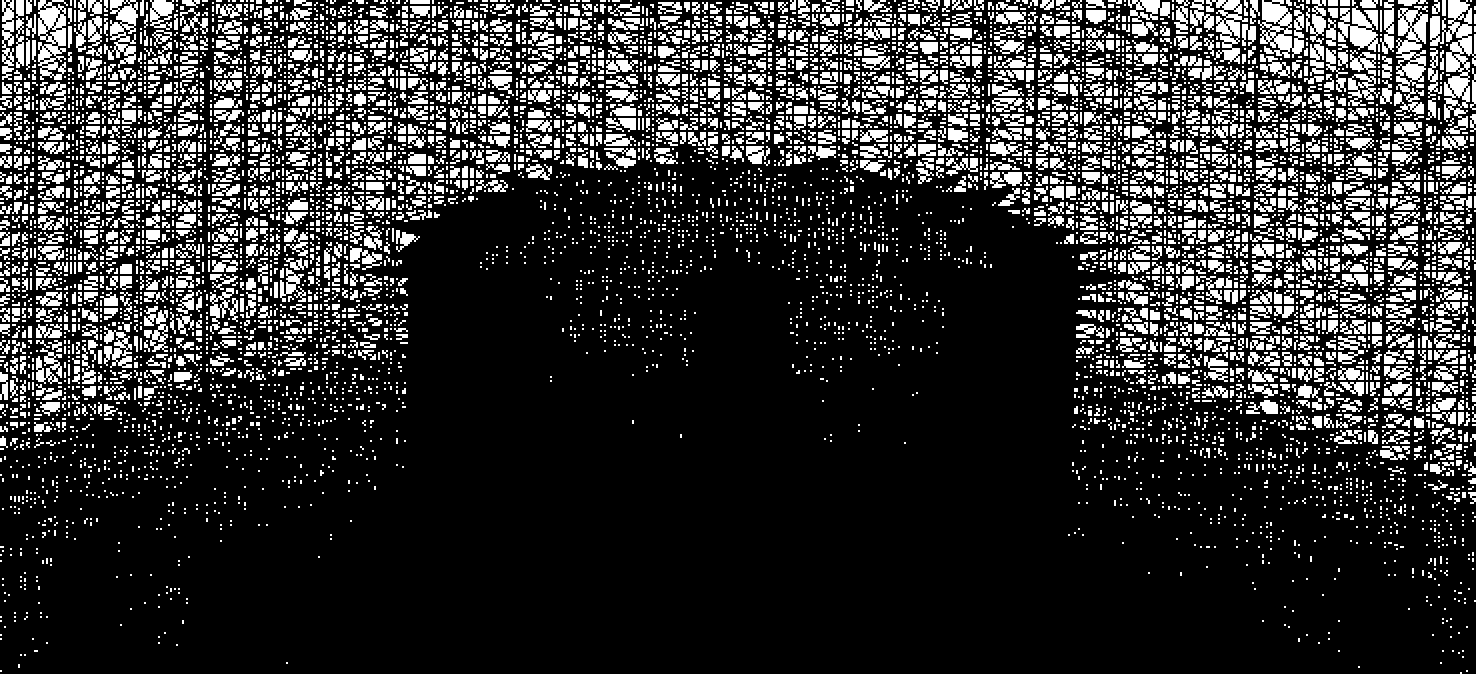
\includegraphics[scale=0.15]{fng_len_tol.png}
    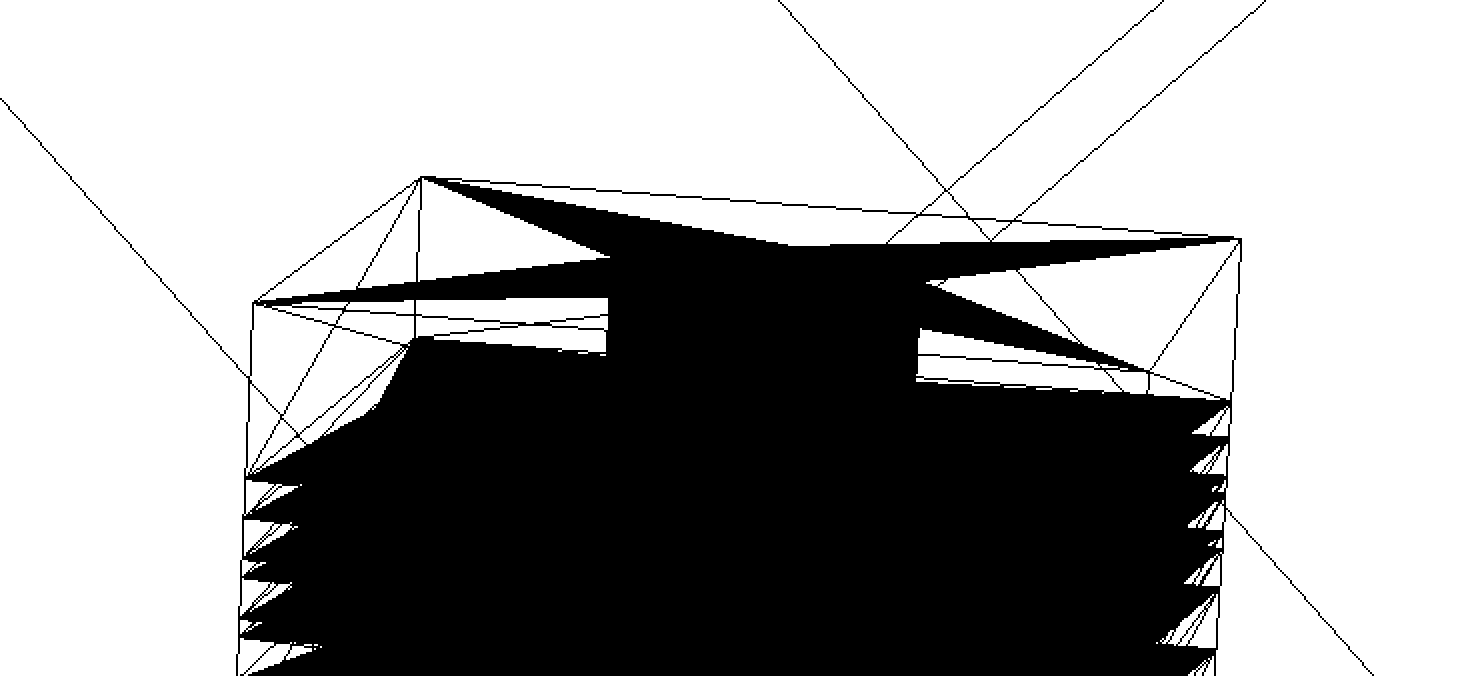
\includegraphics[scale=0.15]{fng_facet_tol.png}
    \caption{The FNG faceted model with (left) and without (right) the length tolerance applied.}
    \label{fng-faceted-models}
  \end{center}

\end{figure}



\subsection{Limitations of the EmDAG system}%%Status:In Progress%%

While the implementation of Embree in DAGMC showed a vast improvement in performance relative to the standard DAGMC implementation, several problems were encountered during the proess. This is not surprising when repurposing a ray tracing kernal for an unintended application.

One of these problems is the presence of lost particles in a watertight model. The FNG model EmDAG was tested on is a fully sealed model via the make\_watertight algorithm. A fully sealed model is one in which every volume is topologically sealed such that there are no gaps between surfaces or adjacent volumes. As a result, DAGMC is able to robustly track particles through such a model with no lost particles. While the lost particle rate for the EmDAG FNG test relatively low, they should not occur at all. After a considerable amount of investigation as to the nature of these lost particles, their cause was determined to be systematic problem not encountered in the nested volume cases. In the DAGMC workflow, a required step for a watertight model is to imprint and merge the surfaces within the CAD system before faceting the model. Imprinting is the process by which CUBIT, the CAD software used to generate DAGMC models, makes surfaces and curves that are coincident in space be fully coincident. This process is accomplished by splitting entities into their coincident and non-coincident parts. The merging process then topologically combines these coincident parts into single entities such that the single entities are topologically adjacent to all entities bounding the original set of entities that were merged into one. The result of these steps is non-manifold model with surfaces shared between neighboring volumes. \cite{smith_thesis_2011} This imprinting and merging of surfaces allows only one representation of each topological entity to be created upon faceting the model. By using the faceted curves of the model as a reference for where surfaces meet in space, the triangles of a surface are made to meet at those curves in a topologically watertight manner. Topologically watertight in reference to triangle facets refers to shared connectivity between surfaces which is distinctly different than watertight by proximity. This topological watertightness of mesh refers to the fact that these surfaces have connectivity at their interface which share vertex handles inside of the MOAB database. These vertex handles will then point to the \textbf{exact same floating point representation} of the vertices no matter which surface is being queried. In this way we do not expect to lose particles through gaps in surfaces and can expect that firing a ray from the logcal position inside a volume should always result in a triangle intersection. This is not the case however when using EmDAG. Particles are somehow being lost in the transport process.

Some detailed debugging of this process revealed that this occurs in a systematic fashion within the FNG model at intersections of 3 or more volumes. The secnario is that a particle moves into the intersection between two surfaces. When this occurs, an intersection with any surface connected to that interface is a valid hit so long as the surface is part of the volume the particle is current positioned within. The particle will then logically move into the volume on the other side of the hit surface. EmDAG handles most of these cases well but for the case in which a particle will have a zero track length inside one of the volumes. A zero track length in this case meaning that the particles trajectory is such that it will only glance the volume without having any appreciable track length inside of it. In this case, the EmDAG system will be unable to find a hit whereas DAGMC's tracking is robust enough to find the triangle intersection on this volume and move on. By isolating this history with a rand card and producing the particle history with locations precise enough to detect the descrepancies between EmDAG and DAGMC, it was found that the position of the particle in EmDAG was numerically too far outside of a volume to produce the correct triangle hit in either EmDAG or DAGMC's ray fire systems. The cause of this descrepancy is believed to have to do with the necessary conversion between double and sinble floating point precision in the EmDAG system. As mentioned before, EmDAG uses single floating point representation in its ray tracing kernel while DAGMC uses a double precision representation of values as does MOAB and MCNP. In order to accomodate Embree's representation, properties of the particle location and direction are converted to single precision for ray tracing queries in Embree and back to double precision when in DAGMC. When changing the floating point representation, rounding rules based on the computing environment are used to determine the new representation according to IEEE standards. \cite{IEEE754_2008} These changes in the particle's location and direction are small, but in the scenario described above it seems that the particle location and/or direction are altered enough throughout the course of its history to cause a missed ray resulting in a lost particle.

In figure \ref{emdag-lost-particles} 

\begin{figure}
  \begin{centering}
  \caption{\textbf{A)} The initial scenario of the lost particle. The particle's trajectory is such that it intersects with the boundary between surfaces A and B. The correct continuation of the particle into volume C is depicted as a dashed line. \textbf{B)} An intersection with surface A is found though either surface A or B are equally valid. The particles position is then updated to its intersection with the boundary of surfaces A and B. The particle then logically moves into volume B. \textbf{C)} Upon establishment of the particle in volume B the Monte Carlo code requests the distance to next surface intersection. The particles position and direction are converted from double to single precision. The small change in the particle's position places it outside of volume B and the trajectory is such that an intersection is not found. At this point the particle is considered lost.}
  \label{emdag-lost-particles}
  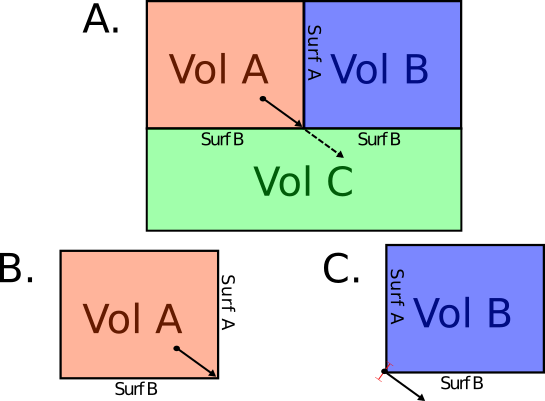
\includegraphics[scale=0.7]{emdag_lost.png}
  \end{centering}
  \end{figure}

In Brandon Smith's thesis Robust Particle Tracking and Advanced Geometry for Monte Carlo Radiation Transport \cite{smith_thesis_2011} there is a detailed description of the different problematic scenarios encountered in tracking particles through a surface mesh representation of a geometric model. Briefly mentioned in this chapter is the possibility of a lost particle due to numerical error in the particle's position perpindicular to the particle's trajectory. Lost paticles caused by this pathology are not handled however as the double floating point representation does not allow the particle position to change enough for this case to occur. In EmDAG, howeve, this case is now vulnerable due to the constant conversion from single to double precision values.

\begin{figure}
  \caption{Example of two adjacent volumes being imprinted and merged.}
\end{figure}


\begin{itemize}
\item Intersection robustness
\item Lost particles due to single to double conversion
\item Limited control over BVH building relative to MOAB
\end{itemize}

\section{Research Proposal}%%Status:In Progress%%
\label{research_proposal}

\subsection{Research Motiviation Summary}%%Status:In Progress%%
In order to make CAD-based Monte Carlo competitive with native codes it is clear that geometry queries must be satistied much more quickly than the ray tracing kernel in DAGMC can currently provide. Investigation into the shortcomings of the DAGMC ray tracing process have revealed various opportunities for improvement. One in implementation and the other in application.

One aspect of these improvements rely on removing the ray tracing kernel from implementation restrictions associated with it being written in the context of a database system and being confined to construction of those database elements. Separation of the kernel allows for a simplified and streamlined system which may be allowed to take advantage of any set of optimizations available in the world of computing. The coupling of DAGMC to Embree provides good evidence of the combination of these assertions. Embree, being an entirely standalone software tool, is inherently free of the databse context in which MOAB's ray tracing tools exist. Additionally, Embree takes advantage of hardware acceleration techniques in the form of single instruction multiple data (SIMD) avilable on most machines.

The Embree ray tracing kernel while very powerful is still oriented toward a rendering application in which a fixed number of primary rays is required to resolve each pixel's color with some secondary rays resulting as dictated by the physics of the model. Similarly, the oriented bounding box (OBB) hierarchy is adapted from a method initially used for interference detection of objects in virtual space. While the application of ray tracing for the purpose of rendering is perhaps closer to the desired application of ray tracing in Monte Carlo than that of interference detection, subtle differences in these applications exist. In optimization, subtleties can greatly impact performance if approached appropriately. One such example in the application of rendering is the recent movement toward firing of rays in packets, taking advantage of the coherency in ray paths coming from a single source. This subtlety is not shared in the realm of Monte Carlo for radiation transport an identical starting condition for a particle can result in a very different pathway through the geometry due to the stochastic nature of a high energy particle's interaction within a medium. It is differences like these that cultivate interest in other properties of Monte Carlo radiation transport that may alter one's approach to design of a ray tracing kernel.

Time it takes to perform the ray tracing queries is partially dependent upon the quality of the acceleration structure being built. The better the quality of these structures is the faster the ray queries will be satisfied and the solution reached. The quality of the accceleration datastructure is also dependent on the amount of time spent in building the datastructures. Presumably the more time spends building the datastructure, the better its quality. Typically, rendering tools focus on building a generalized data structure with respect to the mesh its operating on without consideration of the more subtle features of the mesh and how the datastructure's quality might be improved. This is commonly because the time spent in improving the quality of the datastructure is overly costly compared to the total amount of time saved when performing the ray queries. In the scenario of Monte Carlo, it has been established that many times the number of rays are being fired in order to obtain the solution several times over. In this case the saved time in performing necessary ray queries may then become significant, and that the extra time spend in building the acceleration datastructure to increase its quality becomes favorable. The trade offs of these costs/savings are difficult to quantify in that (as is the case for most ray tracing performance evaluations) they vary greatly model to model. However, the severe degredation in ray fire times due to mesh features produced by the surface mesh generation algorithm on which DAGMC relies leads one to believe that adapting to such mesh features and any other such features discovered in the future is worthwhile.

\subsection{Research Proposal}%%Status:In Progress%%

To address the issues of the implementation context and add mesh adaptive qualities to the BVH build process, a new ray tracing kernel is propsed. This kernel will have components both inside and outside of MOAB. MOAB is currently used to represent DAGMC model topologies as well as their discretized representations. These meshes are generated inside MOAB and as such MOAB has access to alter, manipulate, and query all information about the mesh. It also provides a rich set of mesh manipulation, detection and generation tools. Most importantly, MOAB provides the capability to gaurantee contiguity in memory for both mesh elements and mesh-related data via dense tags. This is a key requirement for many of the efficiencies made available by vectorized operations during traversal of the datastructures. MOAB's unique ability to provide this contiguous data allows one to link its powerful generation, adaptation tools to any set of low-level optimizations available on current CPU architectures. It does not in itself contain the ability to utilize these optimiaztions within its database oriented system, however. As a result, the traversal component of the ray tracing kernel will need to be implemented outside of MOAB. There are a few viable options for accomplishing this. Currently, a system close to this exists inside EmDAG but under the hood Embree is creating its own BVH. It may be possible to structure a BVH from MOAB and pass it to Embree as the data structure to use for traversal. Problems related to the conversion back and forth from double to single precision would need to be addressed as they currently violate the parameters of DADMC's robust particle tracking algorithm and its possible that the particular pathology resulting in lost particles in the EmDAG system is impossible to resolve. Another option is to develop a traversal module either alongside or separate from MOAB which allows for robust raytracing on a double precision triangle surface mesh. This option gives more control over DAGMC in the future in terms of the ability to study different acceleration datastructures, support of specific vector extensions, and a simpler implementation. Embree is an excellent tool with support for many features such as subdivision surfaces, advanced techniques for representation and tracing of hair geometry, etc. which are related more to rendering than they are to ray tracing of static surfaces meshes. 


\subsection{Outline}

\begin{itemize}
\item Reiterate the current state
  \begin{itemize}
  \item Moving outside the database context allows for more freedom of ray tracing implementation, optimization
  \item Facet generation can vary largely and has a significant impact on BVH/OBB performance
  \end{itemize}
\item New take on ray tracing
  \begin{itemize}
  \item Rendering applications of ray tracing do not fret over these small issues because confronting them would significantly increase their time to render/time to solution
  \item Monte Carlo's time to solution is so much longer that the time spent in optimizing a BVH build becomes negligible compared to the additional time spent firing rays (introduce basic equation for tts)
  \item Justified by the fact that we fire more rays in Monte Carlo than in a rendering process (rough estimate of that)
  \end{itemize}
\item Proposed solution
  \begin{itemize}
  \item implementation of a BVH builder supporting many different splitting schemes and SAH leaf condition heuristic
  \item BVH builder will include a registry and solution set for known difficult-to-trace mesh/geometry features
  \item implementation of vectorized ray tracing traversal, taking advantage of MOAB's ability to provide contiguous memory of tag data to create hierarchy
  \item thread-safe kernel which can be used independent of MOAB instance
  \item investigation of available speedup in using different types to define BVH nodes
  \item takes advantage of MOAB's mesh generation capabilities and its ability to provide data in a contiguous set of memory
  \end{itemize}
\item Estimate of performance improvement
  \begin{itemize}
  \item based on current number of ray fires for a sample problem, vectorized implementation, lower precision types, etc.
  \item Use Andrew Turner presentation to project results in context if I'm feeling confident
  \end{itemize}
\end{itemize}

\subsection{Ray Generalization in Radiation Transport}%%Status:Pending%%

Key points to touch on:
\begin{itemize}
\item optimization of time to solution: building time + traversal time
  \begin{itemize}
  \item estimate how long it will take to build BVH?
  \item coarsen BVH build parameters based on estimation of traversal time
  \end{itemize}
\item parallel building of BVH in MOAB
\item mesh feature detection/adaptation during BVH build
  \begin{itemize}
  \item will engineer a system for registering new adaptable features
  \item each feature will have its own response/solution upon detection
  \end{itemize}
\item use of recent heuristics during build
\item vectorized traversal
\item thread-safe kernel for DAGMC and its implications
\item doing this taking advantage of MOAB's intricate/robust mesh interface. then using its direct access to contiguous data for vectorized traversal
\item estimation of improved performance as a result of this work
\end{itemize}


\bibliographystyle{acm}
\bibliography{refs}


\section{Appendix A: Code used to collect data}%%Status:Pending%%
\begin{itemize}
\item ray\_fire\_test program
\end{itemize}

\section{Appendix B: Additional Results}%%Status:In Progress%%

\subsection{Performance Benchmarking Results}%%Status:Done%%

Below lies a set of table containing native MCNP results alongside the DAG-MCNP results for each test case used in doing the performance benchmarking of DAG-MCNP in its current state. These results are not discussed in the main body of this work as they are outside its focus, but they have been provided here for completeness and vaildation of the performance runs.

\begin{table}[H]
  \caption{Results from the FNG run using native MCNP and DAG-MCNP. Flux values are in units of  $cm^{-2}$.}
  \label{fng_perf_results}
  \centering
  \begin{tabular}{l c c}
    \toprule
    Value & MCNP & DAG-MCNP \\
    \hline
    Average Flux Tally & 7.228758E-05 & 7.2278762E-05 \\
    \hline
    Maximum Flux Tally & 1.457239E-04 & 1.4572700E-05 \\
    \hline
    Minimum Flux Tally & 1.997170E-05 & 1.9971600E-05 \\
    \hline
    Average Rel. Error & 4.947389E-04 & 4.947389E-04 \\
    \hline
    Maximum Rel. Error & 8.480259E-04 & 8.480239E-04 \\
    \hline
    Minimum Rel. Error & 3.164050E-04 & 3.164129E-04 \\
    \bottomrule
  \end{tabular}  
\end{table}

\begin{table}[H]
  \centering
  \caption{Results from the UWNR performance test run. Flux values are in units of $cm^{-2}$.}
  \label{uwnr_perf_results}
  \begin{tabular}{l c c}
    \toprule
    Value & MCNP & DAG-MCNP \\
    \hline
    Final $K_{eff}$ & 1.02055 & 1.02095 \\
    \hline
    Average Flux Tally & 1.95320E-01 & 1.94848E-01 \\
    \hline
    Maximum Flux Tally & 4.01669E-01 & 4.05195E-01 \\
    \hline
    Minimum Flux Tally & 5.06464E-02 & 4.87302E-02 \\
    \bottomrule
  \end{tabular}
\end{table}

\begin{table}[H]
  \centering
  \begin{tabular}{l c c}
    \toprule
    Value & MCNP & DAG-MCNP \\
    \hline
    Colliision $K_{eff}$ & 9.9289E-01 &  9.9284E-01 \\
    \hline
    Absorption $K_{eff}$ & 9.9289E-01 & 9.9278E-01 \\
    \hline
    Track Length $K_{eff}$ & 9.9307E-01 & 9.9291E-01 \\
    \hline
    Collision/Absorption $K_{eff}$ & 9.9289E-01 & 9.9282E-01 \\
    \hline
    Absorption/Track Length $K_{eff}$ & 9.9293E-01 & 9.9280E-01 \\
    \hline
    Collision/Track Length $K_{eff}$ & 9.9291E-01 & 9.9285E-01 \\
    \hline 
    Collision/Absorption/Track Length $K_{eff}$ & 9.9291E-01 & 9.9283E-01 \\
    \bottomrule    
  \end{tabular}
\end{table}

\subsection{Additional EmDAG Test Results}%%Status:Pending%%

\subsection{Additional HV WSR Scan Results}%%Status:Pending%%

\end{document}
